\documentclass[dvipsnames]{article}

\usepackage{microtype}
\usepackage{graphicx}
\usepackage{subfigure}
\usepackage{booktabs}

\usepackage{pgfplots} 
\usepackage{xcolor}
\usepackage{tikz}
\usetikzlibrary{positioning, fit, calc, shapes.geometric}
\pgfplotsset{compat=1.18}
\usepackage{amssymb}
\usepackage{pifont}
\newcommand{\Xmark}{\ding{56}}
\newcommand{\Cmark}{\ding{52}}
\newcommand\thingap{\kern 0.2pt}

% Color settings
\def \GuidanceColor             {violet}
    \def \GuidanceDrawColor     {\GuidanceColor!85}
    \def \GuidanceFillColor     {\GuidanceColor!15}
\def \TipColor                  {violet}
    \def \TipDrawColor          {\TipColor!85}
    \def \TipFillColor          {\TipColor!15}
\def \TaskColor                 {BurntOrange}
    \def \TaskDrawColor         {\TaskColor!78!black}
    \def \TaskFillColor         {\TaskColor!10}
\def \AgentActionColor          {NavyBlue}
    \def \AgentActionDrawColor  {\AgentActionColor!90}
    \def \AgentActionFillColor  {\AgentActionColor!10}
\def \ObservationColor          {black}
    \def \ObservationDrawColor  {\ObservationColor!60}
    \def \ObservationFillColor  {\ObservationColor!10}

\tikzset{
    guidance colors/.style={
        fill=\GuidanceFillColor,
        draw=\GuidanceDrawColor,
    },
    tip colors/.style={
        fill=\TipFillColor,
        draw=\TipDrawColor,
    },
    task colors/.style={
        fill=\TaskFillColor,
        draw=\TaskDrawColor,
    },
    action colors/.style={
        fill=\AgentActionFillColor,
        draw=\AgentActionDrawColor,
    },
    observation colors/.style={
        fill=\ObservationFillColor,
        draw=\ObservationDrawColor,
    },
}

\newcommand{\Agent}[1]{
    % #1 = options for the scope
    
    \def\bodyWidth{16pt}
    \def\bodyHeight{3pt}
    \def\headWidth{13pt}
    \def\headOffset{3pt}
    \def\fillColor{NavyBlue!70!gray}
    
    \begin{scope}[#1]
    
        \draw[fill=\fillColor, draw=\fillColor, rounded corners=0.25pt] 
            (0.5pt,0) 
            rectangle (\bodyWidth - 0.5pt, \bodyHeight);
      
        \draw[fill=\fillColor, draw=white, semithick]
            (0, \bodyHeight - 0.05pt) 
            arc [start angle=180, end angle=0, radius=\bodyWidth/2];

        \draw[fill=\fillColor, draw=white, semithick] 
            (\bodyWidth/2, \bodyHeight + \bodyWidth/2 + \headOffset) 
            circle (\headWidth / 2);
        
    \end{scope}
}

\newcommand{\Teacher}[1]{
    \def\BoardOffsetX{-15pt}
    \def\BoardOffsetY{5pt}
    \def\BoardWidth{22pt}
    \def\BoardHeight{18pt}
    \def\PointerColor{Apricot!80!black}

    
    \begin{scope}[#1]
        \draw[fill=black!80, draw=Apricot!80!black, ultra thick, rounded corners]
            (\BoardOffsetX, \BoardOffsetY)
            rectangle (\BoardOffsetX + \BoardWidth, \BoardOffsetY + \BoardHeight);
        \Agent{}
        \draw[fill=\PointerColor, draw=white, ultra thin, shift={(4pt, 2pt)}] 
            (0,0) -- (-12pt,12pt) -- (1pt,1pt) -- cycle;
    \end{scope}
}

\newcommand{\Reviewer}[1]{
    \def\bodyWidth{16pt}
    \def\BridgeWidth{1.5pt}
    \def\BridgeOffsetY{0.8pt}
    \def\FrameOuterRad{2.3pt}
    \def\FrameThickness{0.9pt}
    \def\ArmLength{1.9pt}
    \def\GlassesOffsetX{\bodyWidth/2 - \FrameOuterRad - \BridgeWidth}
    \def\GlassesOffsetY{10.5pt}
    \def\FrameColor{black!80}
    \def\GlassColor{TealBlue!30}

    
    \begin{scope}[#1]
        \Agent{}
        
        \draw[
            fill=\FrameColor,
            draw=none,
            ultra thin,
            shift={(4pt, 2pt)}
        ] (\GlassesOffsetX - \BridgeWidth/2, \GlassesOffsetY) circle (\FrameOuterRad);
            
        \draw[
            fill=\GlassColor,
            draw=none,
            ultra thin,
            shift={(4pt, 2pt)}
        ] (\GlassesOffsetX - \BridgeWidth/2, \GlassesOffsetY) 
            circle (\FrameOuterRad - \FrameThickness);
        
        \draw[
            fill=\FrameColor,
            draw=none,
            ultra thin,
            shift={(4pt, 2pt)},
        ] (\GlassesOffsetX + \FrameOuterRad*2 + \BridgeWidth/2, \GlassesOffsetY)
            circle (\FrameOuterRad);

        \draw[
            fill=\GlassColor,
            draw=none,
            ultra thin,
            shift={(4pt, 2pt)},
        ] (\GlassesOffsetX + \FrameOuterRad*2 + \BridgeWidth/2, \GlassesOffsetY)
            circle (\FrameOuterRad - \FrameThickness);

        % Bridge
        \draw[
            fill=\FrameColor,
            draw=none,
            ultra thin,
        ]   (\GlassesOffsetX  + \FrameOuterRad*2 + \BridgeOffsetY/2, \GlassesOffsetY + \FrameOuterRad + \BridgeOffsetY)
            arc[start angle=135, end angle=45, radius=2pt]
            -- ++(0, -\FrameThickness)
            arc[start angle=45, end angle=135, radius=2pt]
            -- cycle;

        % Arm
        % Сalculations are a mess here
        \draw[
            fill=\FrameColor,
            draw=none,
            ultra thin,
        ]   (\GlassesOffsetX + \FrameThickness*2, \GlassesOffsetY + \FrameOuterRad + \BridgeOffsetY)
            -- ++(-\ArmLength, \ArmLength)
            arc[start angle=45, end angle=180, radius=\FrameOuterRad/2 + \FrameThickness*(1.41/5)]
            % -- ++(\FrameThickness, 0)
            arc[start angle=180, end angle=360, radius=\FrameThickness/2]
            arc[start angle=180, end angle=45, radius=\FrameOuterRad/2 - \FrameThickness/1.6]
            -- ++(\ArmLength, -\ArmLength)
            -- cycle;
        
    \end{scope}
}

\newcommand{\Star}[1]{
    \def\InnerRad{1.5pt}
    \def\OuterRad{3.8pt}
    
    \path[#1] 
        (0  :\OuterRad) -- ( 36:\InnerRad) 
        -- (72 :\OuterRad) -- (108:\InnerRad)
        -- (144:\OuterRad) -- (180:\InnerRad)
        -- (216:\OuterRad) -- (252:\InnerRad)
        -- (288:\OuterRad) -- (324:\InnerRad)--cycle;}


% \newcommand{\oldOverviewFigure}{
    
%     \begin{tikzpicture}[
%         box/.style={
%             draw=black,
%             semithick,
%             rounded corners,
%             font=\scriptsize,
%             align=center,
%             minimum width=20pt,
%         },
%         message/.style={
%             box,
%             text width=43pt,
%         },
%         grade/.style={box, outer xsep=2pt},
%         traj line/.style={
%             thick, rounded corners
%         },
%         prompt/.style={
%             ->, traj line
%         },
%     ]
%         % ========
%         % PHASE 1
%         % ========
            
%         % Prompt
%         \node[
%             message,
%             guidance colors,
%         ] (guidance) {guidance};
%         \node[message, below=5pt of guidance] (task) {\vphantom{p} task};
%         \draw[traj line] (task) -- (guidance);
%         \node[above=8pt of guidance] (phase one) {\vphantom{p} \bfseries \shortstack{Phase 1:\\training data}};
        
%         % Teacher
%         \Teacher{local bounding box=teacher, shift={($(task.south)+(-0.5pt,-34pt)$)}};
%         \node[below=-1pt of teacher] (teacher label) {\scriptsize teacher};
%         \draw[prompt] (task) -- ($(teacher.north)+(0, 2pt)$);

%         % Teacher trajectory
%         \node[message, below=55pt of task]       (t1) {action$\thingap _0$};
%         \node[message, below=6pt of t1]          (t2) {observation$\thingap _1$};
%         \node[message, below=6pt of t2]          (t3) {\ldots};
%         \node[message, below=6pt of t3]          (t4) {observation$\thingap _n$};
%         \node[message, below=6pt of t4]          (t5) {action$\thingap _n$};
%         \node[
%             fit=(t1)(t2)(t3)(t4)(t5),
%             box,
%             densely dashed,
%             inner sep=4pt,
%         ] (teacher traj) {};
%         \draw[>-, traj line]                    (teacher.south) ++ (0pt, -11.5pt) -- (t1);
%         \draw[traj line]                        (t1) -- (t2);
%         \draw[traj line]                        (t2) -- (t3);
%         \draw[traj line]                        (t3) -- (t4);
%         \draw[traj line]                        (t4) -- (t5);

%         % ========
%         % PHASE 2
%         % ========
        
%         % Prompt
%         \node[
%             message,
%             right=52pt of guidance,
%             guidance colors,
%         ] (guidance) {guidance};
%         \node[message, below=5pt of guidance] (task) {\vphantom{p} task};
%         \node[message, below=7pt of task] (t1) {action$\thingap _0$};
%         \node[message, below=5pt of t1] (t2) {\ldots};
%         \node[message, below=5pt of t2] (t3) {observation$\thingap _i$};
%         \node[message, below=5pt of t3] (t4) {action$\thingap _i$};
%         \node[
%             fit=(t1)(t2)(t3)(t4),
%             densely dashed,
%             draw=black,
%             semithick,
%             rounded corners
%         ] (trunk traj) {};
%         \draw[traj line] (task) -- (t1);
%         \draw[traj line] (t1) -- (t2);
%         \draw[traj line] (t2) -- (t3);
%         \draw[traj line] (t3) -- (t4);
%         \draw[traj line, densely dashed, semithick, rounded corners] 
%             (teacher traj.north east) ++ (0, -10pt) 
%             -- ++ (12pt, 0) 
%             |- node[above, anchor=south east, pos=1.02]{\tiny $i=1 \ldots n$} 
%             ($(trunk traj.west)+(0, 0)$);

%         \node[above=8pt of guidance] (phase two) {\vphantom{p} \bfseries \shortstack{Phase 2:\\distillation}};
        
%         % Agents
%         \Agent{local bounding box=student, shift={($(trunk traj.south)+(-42pt,-40pt)$)}};
%         \node[below=-1pt of student] (student label) {\scriptsize student};
%         \draw[prompt]
%             (t4.west) 
%             -| ($(student.north)+(0, 2pt)$);

%         \Teacher{local bounding box=teacher, shift={($(trunk traj.south)+(39pt,-40pt)$)}};
%         \node[below=-1pt of teacher] (teacher label) {\scriptsize teacher};
%         \draw[prompt]
%             (t4.east) 
%             -| ($(teacher.north)+(-2.5pt, 2pt)$);
%         \draw[prompt, draw=\GuidanceDrawColor]
%             (guidance.east)
%             -| ($(teacher.north)+(2.5pt, 2pt)$);

%         % Logits
%         \node[box, below=28pt of student] (student logits) {logits};
%         \draw[prompt, ->] 
%             (student.south) ++ (0pt, -10.5pt) 
%             -- ($(student logits.north)+(0pt, 2pt)$);
%         \node[
%             box,
%             below=28pt of teacher,
%             guidance colors,
%         ] (teacher logits) {logits};
%         \draw[prompt, ->, draw=\GuidanceDrawColor] 
%             (teacher.south) ++ (0pt, -10.5pt) 
%             -- ($(teacher logits.north)+(0pt, 2pt)$);

%         % Loss
%         \node[fit=(student logits)(teacher logits)] (logits) {};
%         \node[box, below=0pt of logits, inner sep=8pt] (loss) {KL Loss};
%         \draw[prompt] (student logits) |- (loss);
%         \draw[prompt, draw=\GuidanceDrawColor] (teacher logits) |- (loss);
%         \draw[prompt, draw=\GuidanceDrawColor] 
%             (loss) |- node[above, pos=0.6] {\scriptsize back-prop} 
%             ($(student.east)+(4pt, 0)$);
%         \Star{
%             draw=\GuidanceColor!70,
%             ultra thin,
%             fill=\GuidanceColor!70,
%             shift={($(student.east)+(11pt, -6pt)$)},
%         }

%         % ========
%         % PHASE 3
%         % ========
        
%         % Reviewer prompt
%         \node[
%             box,
%             right=94pt of guidance.north, 
%             anchor=north,
%         ] (mistake description) {\shortstack{mistake\\description}};

%          % Student prompt
%         \node[
%             message,
%             right=55pt of mistake description.north,
%             anchor=north,
%         ] (task) {\vphantom{p} task};

%         \node[above=10pt of task] (phase three) {\bfseries \shortstack{Phase 3:\\ mistake correction}};
        
%         % Reviewer
%         \Reviewer{
%             local bounding box=reviewer,
%             shift={($(mistake description.south)+(-8pt,-34pt)$)}
%         };
%         \node[below=-1pt of reviewer] (student label) 
%             {\scriptsize \shortstack{LLM-powered\\reviewer}};
%         \draw[prompt] (mistake description) -- ($(reviewer.north)+(0, 2pt)$);
        
%         % Trained student
%         \Agent{local bounding box=student, shift={($(reviewer.south)+(47pt, 0pt)$)}};
%         \Star{
%             draw=white,
%             ultra thin,
%             fill=\GuidanceColor!70,
%             shift={($(student.east)+(-3.5pt, -6pt)$)},
%         };
%         \node[below=-1pt of student] (student label) 
%             {\scriptsize \shortstack{trained\\student}};
%         \draw[prompt] (task) -- ($(student.north)+(0, 2pt)$);

        
%         % Trajectory with mistakes
%         \node[message, below=72pt of task]       (s1) {action$\thingap_0$};
%         \node[message, below=6pt of s1]          (s2) {\ldots};
%         \node[message, below=6pt of s2]          (s3) {observation$\thingap_k$};
%         \node[
%             box,
%             below=14pt of s3,
%             xshift=-20pt,
%             draw=Mahogany!80!Red,
%             fill=Mahogany!10,
%             thick, align=center,
%         ] (s4) {\shortstack{\vphantom{t}wrong\\action$\thingap_k$}};
%         \node[message, below=14pt of s4, xshift=20pt]          (s5) {\ldots};
%         \node[message, below=6pt of s5]          (s6) {action$\thingap_m$};
%         \node[
%             fit=(s1)(s2)(s3),
%             box,
%             dashed,
%             inner sep=4pt,
%             draw=none,
%         ] (student traj) {};
        
%         \draw[>-, traj line]                    (student.south) ++ (0pt, -19.5pt) -- (s1);
%         \draw[traj line]                        (s1) -- (s2);
%         \draw[traj line]                        (s2) -- (s3);
%         \draw[traj line]  
%             (s3.south) -- ++ (0, -5pt) -| (s4);
%         \draw[traj line]                        
%             (s4.south) -- ++ (0, -9pt) -| (s5);
%         \draw[traj line]                        (s5) -- (s6);

%         % Reviewer evaluation
%         \node[grade] (e1) at (mistake description |- s1) {\color{ForestGreen}\Cmark};
%         \node[grade] (e2) at (mistake description |- s2) {\ldots};
%         \node[grade] (e3) at (mistake description |- s3) {\color{ForestGreen}\Cmark};
%         \node[
%             grade,
%             draw=Mahogany!80!Red,
%             thick,
%         ] (e4) at (mistake description |- s4) {\color{Mahogany!80!Red}\Xmark};
%         \node[grade] (e5) at (mistake description |- s5) {\ldots};
%         \node[grade] (e6) at (mistake description |- s6) {\color{ForestGreen}\Cmark};

%         \draw[>-, traj line, dotted]  (reviewer.south) ++ (0pt, -20.5pt) -- (e1);
%         \draw[traj line, dotted] (e1) -- (e2);
%         \draw[traj line, dotted] (e2) -- (e3);
%         \draw[traj line, dotted] (e3) -- (e4);
%         \draw[traj line, dotted] (e4) -- (e5);
%         \draw[traj line, dotted] (e5) -- (e6);

%         \draw[prompt] (s1) -- (e1) ;
%         \draw[prompt] (s2) -- (e2);
%         \draw[prompt] (s3) -- (e3);
%         \draw[prompt] (s4) -- (e4);
%         \draw[prompt] (s5) -- (e5);
%         \draw[prompt] (s6) -- (e6);

%         % Teacher
%         \Teacher{local bounding box=teacher, shift={($(student.south)+(56pt, -82pt)$)}};
%         \Star{
%             draw=white,
%             ultra thin,
%             fill=\GuidanceColor!70,
%             shift={($(teacher.east)+(-3.5pt, -6pt)$)},
%         };
%         \node[below=-1.0pt of teacher, xshift=-0pt] (teacher label) 
%             {\scriptsize \shortstack{teacher}};
%         \draw[prompt] (s3) -- ($(s3 -| teacher.west) + (-3pt, 0)$);

%         % Corrected action
%         \node[
%             box,
%             right=3pt of s4,
%             outer sep=4pt,
%             tip colors,
%             thick,
%         ] (corrected) {\shortstack{\vphantom{p}improved\\action$\thingap_k$}};
%         \draw[prompt, -] 
%             ($(teacher label.south) + (-4pt, 0.5pt)$) 
%             |- ($(corrected.east) + (-4pt, 0)$); 

%         \draw[
%             draw=black,
%             densely dashed,
%             semithick, 
%             rounded corners,
%         ]
%             (student traj.north west) 
%             -- (student traj.south west |- corrected.north west)
%             -- (corrected.north west)
%             -- (corrected.south west)
%             -- (corrected.south east)
%             -- (corrected.north east)
%             -- (student traj.south east |- corrected.north east)
%             -- (student traj.north east) 
%             -- (student traj.north west);

%         % Tip
%         \node[
%             box,
%             above=32pt of teacher label,
%             xshift=-4pt,
%             tip colors,
%         ] (tip) {\shortstack{tip}};
%         \draw[prompt, rounded corners=3pt] (tip.south) -- ++ (0, -3pt)
%         -| ($(teacher label.north)+(-4pt, 25pt)$);

%         % ========
%         % PHASE 4
%         % ========

%         % Student trajectory
%         \node[message, right=92pt of task]    (s1) {action$\thingap _0$};
%         \node[message, below=6pt of s1]    (s2) {\ldots};
%         \node[message, below=6pt of s2]    (s3) {observation$\thingap _k$};
%         \node[
%             message,
%             below=8pt of s3,
%             tip colors,
%             thick,
%         ] (corrected copy) {\shortstack{improved\\action$\thingap _k$}};
%         \node[
%             box,
%             right=14pt of corrected copy,
%             tip colors,
%         ] (tip) {\strut tip};
%         \node[
%             fit=(s1)(s2)(s3)(corrected copy),
%             box,
%             densely dashed,
%             inner sep=4pt,
%         ] (traj) {};
%         \draw[densely dashed, semithick, rounded corners] 
%             (student traj.east) ++ (0, 22pt)
%             -- ++ (8pt,0pt)
%             |- ($(traj.west)+(0,-16pt)$);

%         \draw[traj line]        (s1) -- (s2);
%         \draw[traj line]        (s2) -- (s3);
%         \draw[traj line]        (s3) -- (corrected copy);

%         \node[above=8pt of s1] (phase four) {\vphantom{p} \bfseries \shortstack{Phase 4:\\distilling corrections}};
        
%         % Agents
%         \Agent{local bounding box=student, shift={($(corrected copy.south)+(-42pt,-40pt)$)}};
%         \Star{
%             draw=white,
%             ultra thin,
%             fill=\GuidanceColor!70,
%             shift={($(student.east)+(-3.5pt, -6pt)$)},
%         }
%         \node[below=-1pt of student] (student label) {\scriptsize student};
%         \draw[prompt]
%             (corrected copy.west) 
%             -| ($(student.north)+(0, 2pt)$);

%         \Teacher{local bounding box=teacher, shift={($(corrected copy.south)+(39pt,-40pt)$)}};
%         \Star{
%             draw=white,
%             ultra thin,
%             fill=\GuidanceColor!70,
%             shift={($(teacher.east)+(-3.5pt, -7pt)$)},
%         }
%         \node[below=-1pt of teacher] (teacher label) {\scriptsize teacher};
%         \draw[prompt]
%             (corrected copy.east) 
%             -| ($(teacher.north)+(-5.5pt, 2pt)$);
%         \draw[prompt, draw=\TipDrawColor]
%             (tip.south) -- ++ (0, -6pt)
%             -| ($(teacher.north)+(-0.5pt, 2pt)$);

%         % Logits
%         \node[box, below=28pt of student] (student logits) {logits};
%         \draw[prompt, ->] 
%             (student.south) ++ (0pt, -10.5pt) 
%             -- ($(student logits.north)+(0pt, 2pt)$);
%         \node[
%             box,
%             below=28pt of teacher,
%             tip colors,
%         ] (teacher logits) {logits};
%         \draw[prompt, ->, draw=\TipDrawColor] 
%             (teacher.south) ++ (0pt, -10.5pt) 
%             -- ($(teacher logits.north)+(0pt, 2pt)$);

%         % Loss
%         \node[fit=(student logits)(teacher logits)] (logits) {};
%         \node[box, below=0pt of logits, inner sep=7pt] (loss) {KL Loss};
%         \draw[prompt] (student logits) |- (loss);
%         \draw[prompt, draw=\TipDrawColor] (teacher logits) |- (loss);
%         \draw[prompt, draw=\TipDrawColor] 
%             (loss) |- node[above, pos=0.6] {\scriptsize back-prop} 
%             ($(student.east)+(4pt, 0)$);
        
        
%     \end{tikzpicture}
% }

\newcommand{\roundOne}{
    
    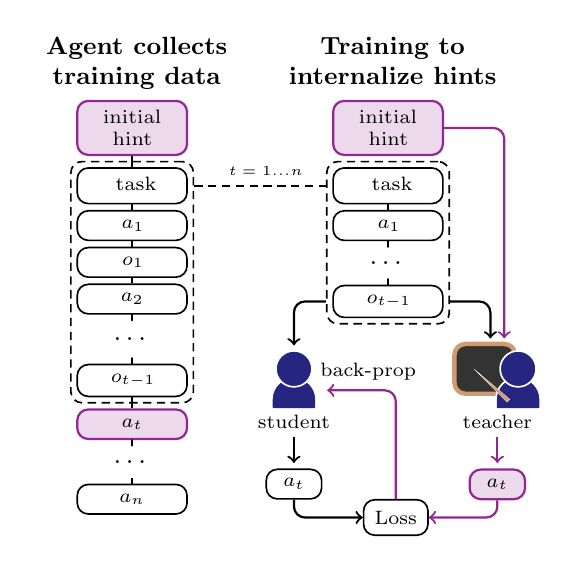
\begin{tikzpicture}[
        box/.style={
            draw=black,
            semithick,
            rounded corners,
            font=\scriptsize,
            align=center,
            minimum width=20pt,
        },
        message/.style={
            box,
            text width=33pt,
        },
        grade/.style={box, outer xsep=2pt},
        traj line/.style={
            thick, rounded corners
        },
        prompt/.style={
            ->, traj line
        },
    ]
        % ========
        % PHASE 1
        % ========
            
        % Prompt
        \node[
            message,
            guidance colors,
            thick,
        ] (guidance) {initial hint};
        \node[message, below=4pt of guidance] (task) {\vphantom{p} task};
        \draw[traj line] (task) -- (guidance);
        \node[above=0pt of guidance] (phase one) {\vphantom{p} \small\bfseries \shortstack{Agent collects\\training data}};
        
        % Teacher trajectory
        \node[message, below=2pt of task]       (t1) {$a_1$};
        \node[message, below=2pt of t1]          (t2) {$o_1$};
        \node[message, below=2pt of t2]       (t21) {$a_2$};

        \node[below=2pt of t21, outer ysep=3pt]          (t22) {\ldots};
        \node[message, below=2pt of t22]          (t23) {$o_{t-1}$};
        \node[
            message,
            below=4pt of t23,
            guidance colors,
            thick,
        ]          (t24) {$a_t$};

        \node[below=2pt of t24, outer ysep=2pt]          (t3) {\ldots};
        % \node[message, below=2pt of t3]          (t4) {$o_{n-1}$};
        \node[message, below=2pt of t3]          (t5) {$a_n$};
        \node[
            fit=(task)(t1)(t2)(t21)(t22)(t23),
            box,
            densely dashed,
            inner sep=2pt,
        ] (teacher traj) {};
        \draw[traj line]                        (task) -- (t1);
        \draw[traj line]                        (t1) -- (t2);
        \draw[traj line]                        (t2) -- (t21);
        \draw[traj line, line cap=round]        (t21) -- (t22);
        \draw[traj line, line cap=round]        (t22) -- (t23);
        \draw[traj line]                        (t23) -- (t24);
        \draw[traj line, line cap=round]        (t24) -- (t3);
        % \draw[traj line, line cap=round]        (t3) -- (t4);
        \draw[traj line]                        (t3) -- (t5);

        % ========
        % PHASE 2
        % ========
        
        % Prompt
        \node[
            message,
            right=52pt of guidance,
            guidance colors,
            thick,
        ] (guidance) {initial hint};
        \node[message, below=4pt of guidance] (task) {\vphantom{p} task};
        \node[message, below=2pt of task] (t1) {$a_1$};
        \node[below=2pt of t1, outer ysep=2pt] (t2) {\ldots};
        \node[message, below=2pt of t2] (t4) {$o_{t-1}$};
        \node[
            fit=(task)(t1)(t2)(t4),
            densely dashed,
            draw=black,
            semithick,
            rounded corners,
            inner sep=2pt,
        ] (trunk traj) {};
        \draw[traj line] (task) -- (t1);
        \draw[traj line, line cap=round] (t1) -- (t2);
        \draw[traj line, line cap=round] (t2) -- (t4);
        \draw[traj line, densely dashed, semithick, rounded corners] 
            (teacher traj.north east |- task.west) 
            -- node[above, anchor=south east, pos=0.9]{\tiny $t=1 ... n$} 
            (trunk traj.west |- task.west);

        \node[above=0pt of guidance] (phase two) {\vphantom{p} \small\bfseries \shortstack{Training to\\internalize hints}};
        
        % Agents
        \Agent{local bounding box=student, shift={($(trunk traj.south)+(-42pt,-30pt)$)}};
        \node[below=-1pt of student] (student label) {\scriptsize student};
        \draw[prompt]
            (trunk traj.west |- t4.west) 
            -| ($(student.north)+(0, 2pt)$);

        \Teacher{local bounding box=teacher, shift={($(trunk traj.south)+(39pt,-30pt)$)}};
        \node[below=-1pt of teacher] (teacher label) {\scriptsize teacher};
        \draw[prompt]
            (trunk traj.east |- t4.east) 
            -| ($(teacher.north)+(-2.5pt, 2pt)$);
        \draw[prompt, draw=\GuidanceDrawColor]
            (guidance.east)
            -| ($(teacher.north)+(2.5pt, 2pt)$);

        % Logits
        \node[box, below=22pt of student] (student logits) {$a_t$};
        \draw[prompt, ->] 
            (student.south) ++ (0pt, -10.5pt) 
            -- ($(student logits.north)+(0pt, 2pt)$);
        \node[
            box,
            below=22pt of teacher,
            guidance colors,
            thick,
        ] (teacher logits) {$a_t$};
        \draw[prompt, ->, draw=\GuidanceDrawColor] 
            (teacher.south) ++ (0pt, -10.5pt) 
            -- ($(teacher logits.north)+(0pt, 2pt)$);

        % Loss
        \node[fit=(student logits)(teacher logits)] (logits) {};
        \node[box, below=-4pt of logits, inner sep=4pt] (loss) {Loss};
        \draw[prompt] (student logits) |- (loss);
        \draw[prompt, draw=\GuidanceDrawColor] (teacher logits) |- (loss);
        \draw[prompt, draw=\GuidanceDrawColor] 
            (loss) |- node[above, pos=0.7] {\scriptsize back-prop} 
            ($(student.east)+(4pt, -4pt)$);
        % \Star{
        %     draw=\GuidanceColor!70,
        %     ultra thin,
        %     fill=\GuidanceColor!70,
        %     shift={($(student.east)+(11pt, -6pt)$)},
        % }

    \end{tikzpicture}

}


\newcommand{\roundTwo}{
    
    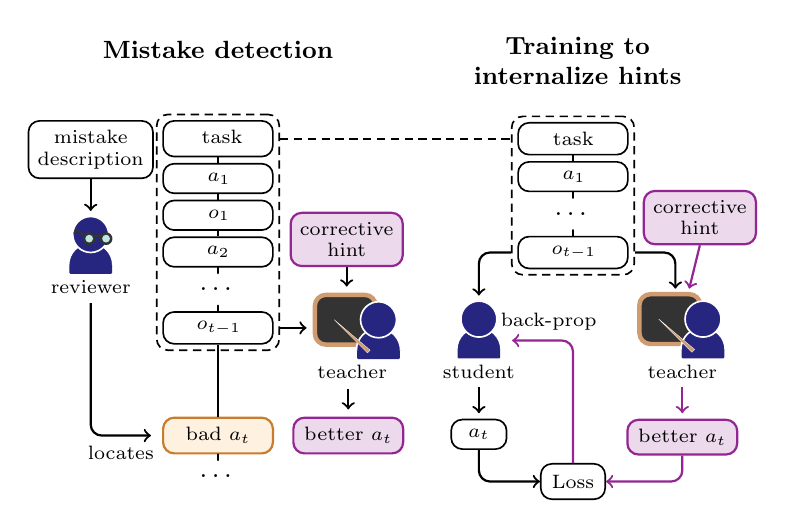
\begin{tikzpicture}[
        box/.style={
            draw=black,
            semithick,
            rounded corners,
            font=\scriptsize,
            align=center,
            minimum width=20pt,
        },
        message/.style={
            box,
            text width=33pt,
        },
        grade/.style={outer xsep=2pt},
        traj line/.style={
            thick, rounded corners
        },
        prompt/.style={
            ->, traj line
        },
    ]

        % Reviewer prompt
        \node[
            box,
            % right=94pt of guidance.north, 
            anchor=north,
        ] (mistake description) {\shortstack{mistake\\description}};

         % Student prompt
        \node[
            message,
            right=46pt of mistake description.north,
            % shift={($(0pt,-54pt)$)},
            anchor=north,
        ] (task) {\vphantom{p} task};

        \node[above=10pt of task] (phase three) {\small\bfseries \shortstack{Mistake detection\\ \vphantom{p}}};
        
        % Reviewer
        \Reviewer{
            local bounding box=reviewer,
            shift={($(mistake description.south)+(-8pt,-34pt)$)}
        };
        \node[below=-1pt of reviewer] (reviewer label) 
            {\scriptsize \shortstack{reviewer}};
        \draw[prompt] (mistake description) -- ($(reviewer.north)+(0, 2pt)$);
        
        
        % Trajectory with mistakes
        \node[message, below=2pt of task]       (s1) {$a_1$};
        \node[message, below=2pt of s1]       (s11) {$o_1$};
        \node[message, below=2pt of s11]       (s12) {$a_2$};
        \node[below=2pt of s12, outer ysep=2pt]          (s2) {\ldots};
        \node[message, below=2pt of s2]          (s3) {$o_{t-1}$};
        \node[
            message, below=26pt of s3,
            task colors,
            thick,
        ] (s4) {\vphantom{hp}bad $a_t$};
        \node[below=2pt of s4, outer ysep=2pt]          (s5) {\ldots};
        % \node[message, below=6pt of s5]          (s6) {$a_n$};
        \node[
            fit=(task)(s1)(s11)(s12)(s3),
            box,
            densely dashed,
            inner sep=2pt,
        ] (teacher traj) {};
        
        \draw[traj line]                        (task) -- (s1);
        \draw[traj line]                        (s1) -- (s11);
        \draw[traj line]                        (s11) -- (s12);
        \draw[traj line, line cap=round]        (s12) -- (s2);
        \draw[traj line, line cap=round]        (s2) -- (s3);
        \draw[traj line]                        (s3) -- (s4);
        \draw[traj line, line cap=round]        (s4) -- (s5);
        % \draw[traj line]                      (s5) -- (s6);

        \draw[traj line, ->] 
            (reviewer label.south) |- node[below, pos=0.75] {\scriptsize locates}
            ($(s4.west) + (-4pt, 0)$);

        % Teacher
        \Teacher{local bounding box=teacher, anchor=south, shift={($(s3.south)+(50pt, -5pt)$)}};
        \node[below=-1.0pt of teacher, xshift=-2pt] (teacher label) 
            {\scriptsize \shortstack{teacher}};
        \draw[prompt] 
            (teacher traj.east |- s3) 
            -- ($(s3 -| teacher.west) + (-3pt, 0)$);

        % Corrected action
        \node[
            message,
            right=4pt of s4,
            outer sep=3pt,
            tip colors,
            thick,
        ] (corrected) {\vphantom{p}better $a_t$};
        \draw[prompt, ->] 
            (corrected |- teacher label.south) -- (corrected); 

        % Tip
        \node[
            box,
            above=32pt of teacher label,
            xshift=-2pt,
            tip colors,
            thick,
        ] (tip) {\shortstack{corrective\\hint}};
        \draw[prompt, rounded corners=3pt] (tip.south)
        -- ($(teacher label.north)+(-2pt, 25pt)$);

        % ========
        % PHASE 4
        % ========

        % Student trajectory
        \node[message, right=88pt of task]       (task) {task};
        \node[message, below=2pt of task]    (s1) {$a_1$};
        \node[below=2pt of s1, outer ysep=2pt]    (s2) {\ldots};
        \node[message, below=2pt of s2]    (s3) {$o_{t-1}$};
        \node[
            box,
            right=15.0pt of s2,
            yshift=-1.3pt,
            tip colors,
            thick,
        ] (tip) {\shortstack{corrective\\hint}};
        \node[
            fit=(task)(s1)(s2)(s3),
            box,
            densely dashed,
            inner sep=2pt,
        ] (traj) {};
        \draw[densely dashed, semithick] 
            (teacher traj.north east |- task.west)
            -- (traj.west |- task.west);

        \draw[traj line]        (task) -- (s1);
        \draw[traj line, line cap=round]        (s1) -- (s2);
        \draw[traj line, line cap=round]        (s2) -- (s3);

        \node[above=8pt of task] (phase four) {\vphantom{p} \small\bfseries \shortstack{Training to\\internalize hints}};
        
        % Agents
        \Agent{local bounding box=student, shift={($(s3.south)+(-42pt,-32pt)$)}};
        \node[below=-1pt of student] (student label) {\scriptsize student};
        \draw[prompt]
            (traj.west |- s3.west) 
            -| ($(student.north)+(0, 2pt)$);

        \Teacher{local bounding box=teacher, shift={($(s3.south)+(39pt,-32pt)$)}};
        \node[below=-1pt of teacher] (teacher label) {\scriptsize teacher};
        \draw[prompt]
            (traj.east |- s3.east) 
            -| ($(teacher.north)+(-2.5pt, 2pt)$);
        \draw[prompt, draw=\TipDrawColor]
            (tip.south) -- ($(teacher.north)+(2.5pt, 2pt)$);

        % Logits
        \node[box, below=22pt of student] (student logits) {$a_t$};
        \draw[prompt, ->] 
            (student.south) ++ (0pt, -10.5pt) 
            -- ($(student logits.north)+(0pt, 2pt)$);
        \node[
            message,
            below=22pt of teacher,
            tip colors,
            thick,
        ] (teacher logits) {better $a_t$};
        \draw[prompt, ->, draw=\TipDrawColor] 
            (teacher.south) ++ (0pt, -10.5pt) 
            -- ($(teacher logits.north)+(0pt, 2pt)$);

        % Loss
        \node[fit=(student logits)(teacher logits)] (logits) {};
        \node[box, below=70pt of s3, inner sep=4pt] (loss) {Loss};
        \draw[prompt] (student logits) |- (loss);
        \draw[prompt, draw=\TipDrawColor] (teacher logits) |- (loss);
        \draw[prompt, draw=\TipDrawColor] 
            (loss) |- node[above, pos=0.7] {\scriptsize back-prop} 
            ($(student.east)+(4pt, -4pt)$);
        
        
    \end{tikzpicture}
}


\newcommand{\trainingCycle}{
    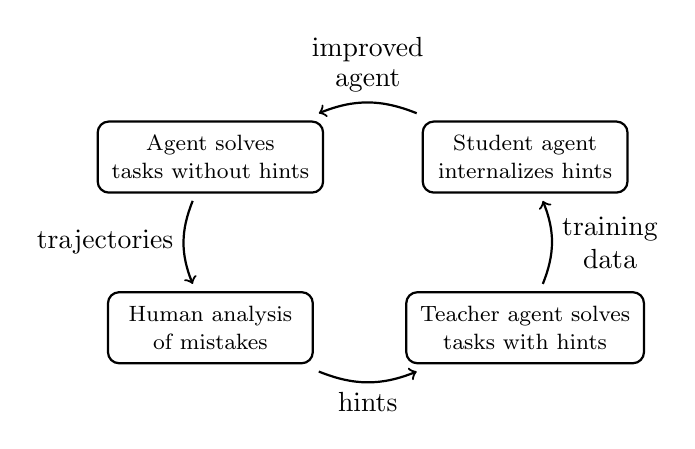
\begin{tikzpicture}[
        box/.style={
            thick,
            draw=black,
            rounded corners,
            inner sep=5pt,
            outer sep=3pt,
            font=\footnotesize,
            minimum width=74pt,
        },
        connection/.style={
            ->,
            thick,
            bend right=22,
        },
        node distance = 30pt,
    ]

        \def \radius {75pt}
        \def \offset {0.08}

        \node[box] (1) {
            \shortstack{Teacher agent solves\\tasks with hints}
        };
        \node[box, above=of 1] (2) {
            \shortstack{Student agent\\internalizes hints}
        };
        \node[box, left=of 2] (3) {
            \shortstack{Agent solves\\tasks without hints}
        };
        \node[box, below=of 3] (4) {
            \shortstack{Human analysis\\of mistakes}
        };

        \path (1) edge[connection] node[right] {\shortstack{training\\data}} (2);
        \path (2) edge[connection] node[above] {\shortstack{improved\\agent}} (3);
        \path (3) edge[connection] node[left] {\shortstack{trajectories}} (4);
        \path (4) edge[connection] node[below] {\shortstack{hints}} (1);
        
    \end{tikzpicture}
}


\newcommand{\mistakeAndHintExample}{
    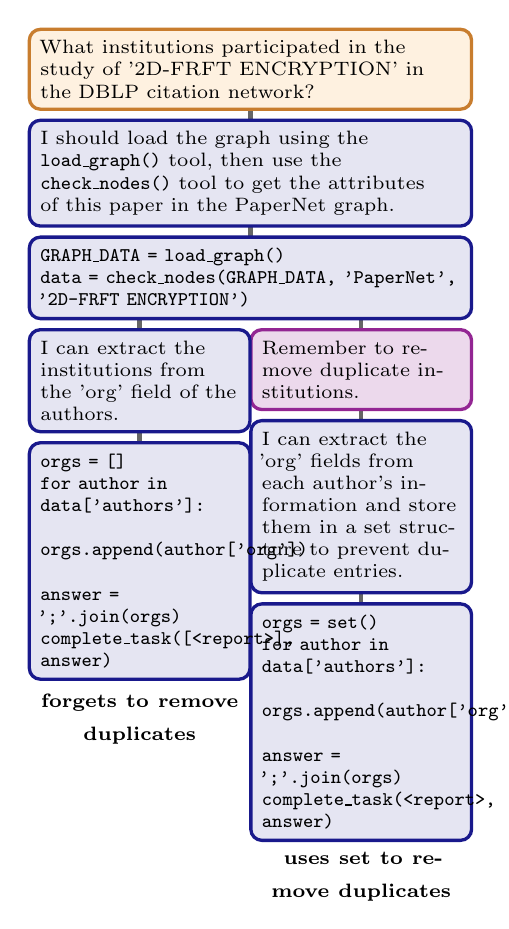
\begin{tikzpicture}[
        message/.style={
            rounded corners,
            very thick,
            inner sep=4pt,
            outer sep=0pt,
            align=left,
            text width=0.208 * \textwidth, font=\scriptsize
        },
    ]
        \pgfdeclarelayer{background}
        \pgfsetlayers{background,main}
        
        % Prompt
        \node[
            message,
            text width=0.44 * \textwidth,
            task colors,
            % align=center,
        ] (task) {What institutions participated in the study of '2D-FRFT ENCRYPTION' in the DBLP citation network?};

        \node[
            message,
            below=4pt of task,
            text width=0.44 * \textwidth,
            action colors,
            % align=center,
        ] (inner monologue) {I should load the graph using the \texttt{load\_graph()} tool, then use the \texttt{check\_nodes()} tool to get the attributes of this paper in the PaperNet graph.};
        \begin{pgfonlayer}{background}
            \draw[ultra thick, draw=black!60] 
                (task) -- (inner monologue);
        \end{pgfonlayer}

        \node[
            message,
            below=4pt of inner monologue,
            text width=0.44 * \textwidth,
            action colors,
            font=\scriptsize \ttfamily,
        ] (action) {
            GRAPH\_DATA = load\_graph() \\
            data = check\_nodes(GRAPH\_DATA, 'PaperNet', '2D-FRFT ENCRYPTION')
        };
        \begin{pgfonlayer}{background}
            \draw[ultra thick, draw=black!60] 
                (inner monologue) -- (action);
        \end{pgfonlayer}

         % Good trajectory
        \node[
            message,
            below=4pt of action.south east,
            tip colors,
            anchor=north east,
        ] (r1) {Remember to remove duplicate institutions.};
        \begin{pgfonlayer}{background}
            \draw[ultra thick, draw=black!60] (r1.north) 
                -- (r1.north |- action.south);
        \end{pgfonlayer}

        \node[
            message,
            below=4pt of r1,
            action colors,
        ] (r2) {I can extract the 'org' fields from each author's information and store them in a set structure to prevent duplicate entries.};
        \begin{pgfonlayer}{background}
            \draw[ultra thick, draw=black!60] (r2) -- (r1);
        \end{pgfonlayer}

        \node[
            message,
            below=4pt of r2,
            action colors,
            font=\scriptsize \ttfamily
        ] (r3) {
            \textbf{orgs = set()} \\
            for author in data['authors']: \\
            \quad orgs.append(author['org']) \\
            \vphantom{p}\\
            answer = ';'.join(orgs) \\
            complete\_task(<report>, answer)
        };
        \begin{pgfonlayer}{background}
            \draw[ultra thick, draw=black!60] (r3) -- (r2);
        \end{pgfonlayer}

        \node[
            align=center,
            text width=0.25 * \textwidth,
            below=4pt of r3,
            inner sep=0pt,
            % scale=0.9,
            % draw=red,
        ] {\scriptsize \bfseries uses set to remove duplicates};

        % Bad trajectory
        \node[
            message,
            below=4pt of action.south west,
            action colors,
            anchor=north west,
        ] (l1) {I can extract the institutions from the 'org' field of the authors.};
        \begin{pgfonlayer}{background}
            \draw[ultra thick, draw=black!60] (l1.north) 
            -- (l1.north |- action.south);
        \end{pgfonlayer}

        \node[
            message,
            below=4pt of l1,
            action colors,
            font=\scriptsize \ttfamily,
        ] (l2) {
            orgs = [] \\
            for author in data['authors']: \\
            \quad orgs.append(author['org']) \\
            \vphantom{p}\\
            answer = ';'.join(orgs) \\
            complete\_task([<report>], answer)
        };
        \begin{pgfonlayer}{background}
            \draw[ultra thick, draw=black!60]
                (l2.north) -- (l1.south);
        \end{pgfonlayer}

        \node[
            align=center,
            % draw=red,
            inner sep=0pt,
            text width=0.22 * \textwidth,
            below=5pt of l2,
            % scale=0.9,
        ] {\scriptsize \bfseries forgets to remove duplicates};

    \end{tikzpicture}
}

\newcommand{\exampleTrajectoryDiagram}{
    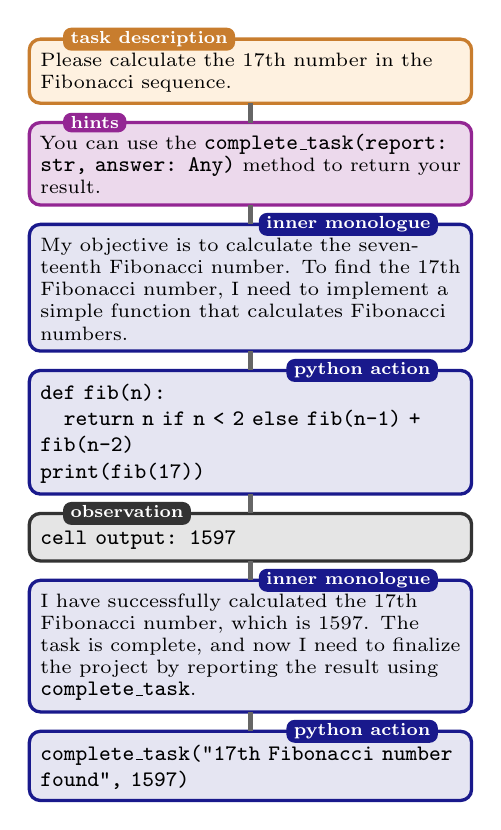
\begin{tikzpicture}[
        legend item/.style={very thick, minimum height=10pt, minimum width=10pt},
        message/.style={font=\scriptsize, rounded corners, very thick, inner sep=4pt, outer sep=0, align=left, text width = 0.44 * \textwidth},
        fancy title/.style={font=\scriptsize\bfseries, rounded corners=3pt, right=12pt, text=white, inner xsep=3pt, inner ysep=1.5pt, scale=0.9},
        node distance=7pt,
    ]
        % Task description 
        \node[message, task colors] (m1) {\vphantom{A} \\ [-7pt]
        Please calculate the 17th number in the Fibonacci sequence.};
        \node[fancy title, fill=\TaskDrawColor] at (m1.north west) (t1) {task description};

        % Guidance
        \node[message, tip colors, below=of m1] (m2) {\vphantom{A} \\ [-7pt]
        You can use the \texttt{\footnotesize complete\_task(report: str, answer: Any)} method to return your result.};
        \node[fancy title, fill=\TipDrawColor] at (m2.north west) (t2) {hints};
        \draw[line width=2.0pt, draw=black!60] (m1) -- (m2);

        % Inner monologue 1
        \node[message, action colors, below=of m2] (m3) {\vphantom{A} \\ [-7pt] 
        My objective is to calculate the seventeenth Fibonacci number. To find the 17th Fibonacci number, I need to implement a simple function that calculates Fibonacci numbers.};
        \node[fancy title, fill=\AgentActionDrawColor, right=-12pt, anchor=east] at (m3.north east) (t3) {inner monologue};
        \draw[line width=2.0pt, draw=black!60] (m2) -- (m3);

        % Python 1
        \node[message, font=\footnotesize\ttfamily, action colors, below=of m3] (m4) {\vphantom{A} \\ [-8pt] 
        def fib(n):\\
        \quad return n if n < 2 else fib(n-1) + fib(n-2)\\
        % \vphantom{A}\\
        print(fib(17))};
        \node[fancy title, fill=\AgentActionDrawColor, right=-12pt, anchor=east] at (m4.north east) (t4) {python action};
        \draw[line width=2.0pt, draw=black!60] (m3) -- (m4);

         % Output 1
        \node[message, font=\footnotesize\ttfamily, draw=black!80, fill=black!10, below=of m4] (m5) {\vphantom{A} \\ [-7pt] 
        cell output: 1597};
        \node[fancy title, fill=black!80] at (m5.north west) (t5) {\vphantom{p}observation};
        \draw[line width=2.0pt, draw=black!60] (m4) -- (m5);

        % Inner monologue 2
        \node[message, draw=NavyBlue!90, fill=NavyBlue!10, below=of m5] (m6) {\vphantom{A} \\ [-7pt] 
        I have successfully calculated the 17th Fibonacci number, which is 1597. The task is complete, and now I need to finalize the project by reporting the result using \texttt{\footnotesize complete\_task}.};
        \node[fancy title, fill=NavyBlue!90, right=-12pt, anchor=east] at (m6.north east) (t6) {inner monologue};
        \draw[line width=2.0pt, draw=black!60] (m5) -- (m6);

        % Python 2
        \node[message, action colors, below=of m6, font=\footnotesize\ttfamily] (m7) {\vphantom{A} \\ [-8pt] 
            complete\_task("17th Fibonacci number found", 1597)};
        \node[fancy title, fill=\AgentActionDrawColor, right=-12pt, anchor=east] at (m7.north east) (t7) {python action};
        \draw[line width=2.0pt, draw=black!60] (m6) -- (m7);
        
    \end{tikzpicture}
}






\usepackage{hyperref}

\newcommand{\theHalgorithm}{\arabic{algorithm}}

\usepackage[accepted]{arxiv_preprint}

\usepackage{amsmath}
\usepackage{amssymb}
\usepackage{mathtools}
\usepackage{amsthm}
\usepackage{array}

\usepackage[capitalize,noabbrev]{cleveref}

\usepackage{multirow}
\usepackage{pifont}
\newcommand{\cmark}{\ding{51}}
\newcommand{\xmark}{\ding{55}}

\theoremstyle{plain}
\newtheorem{theorem}{Theorem}[section]
\newtheorem{proposition}[theorem]{Proposition}
\newtheorem{lemma}[theorem]{Lemma}
\newtheorem{corollary}[theorem]{Corollary}
\theoremstyle{definition}
\newtheorem{definition}[theorem]{Definition}
\newtheorem{assumption}[theorem]{Assumption}
\theoremstyle{remark}
\newtheorem{remark}[theorem]{Remark}

\usepackage{listings}
\usepackage[scaled=.87]{inconsolata}
\definecolor{LightGray}{gray}{0.95}
\newcommand{\mytt}[1]{\texttt{#1}}

\lstdefinestyle{custom}{
  breaklines=true,
  basicstyle=\fontsize{8pt}{8pt}\ttfamily,
  backgroundcolor=\color{LightGray},
  columns=fullflexible,
  showstringspaces=false,
  breakindent=0pt,
  xleftmargin=3pt,
  framesep=3pt,
  frame=leftline,
  rulecolor=\color{LightGray},
  postbreak=\mbox{$\hookrightarrow$\space\space}
}
\lstset{style=custom}


\icmltitlerunning{Coaching AI Agents to Master Multiple Tasks via Hints Internalization}
\begin{document}

\twocolumn[

\icmltitle{Memento No More: Coaching AI Agents\\ to Master Multiple Tasks via Hints Internalization}

\icmlsetsymbol{equal}{*}

\begin{icmlauthorlist}
\icmlauthor{Minttu Alakuijala}{equal,yyy}
\icmlauthor{Ya Gao}{equal,yyy}
\icmlauthor{Georgy Ananov}{yyy}
\icmlauthor{Samuel Kaski}{yyy} \\
\icmlauthor{Pekka Marttinen}{yyy}
\icmlauthor{Alexander Ilin}{comp}
\icmlauthor{Harri Valpola}{comp}
\end{icmlauthorlist}

\icmlaffiliation{yyy}{Department of Computer Science, Aalto University}
\icmlaffiliation{comp}{System 2 AI}

\icmlcorrespondingauthor{Minttu Alakuijala}{minttu.alakuijala@aalto.fi}
\icmlcorrespondingauthor{Ya Gao}{ya.gao@aalto.fi}

\icmlkeywords{Large Language Models, Distillation, LLM Agents}

\vskip 0.3in
]

\printAffiliationsAndNotice{\icmlEqualContribution}

\begin{abstract}
As the general capabilities of artificial intelligence (AI) agents continue to evolve, their ability to learn to master multiple complex tasks through experience remains a key challenge. Current LLM agents, particularly those based on proprietary language models, typically rely on prompts to incorporate knowledge about the target tasks. This approach does not allow the agent to \emph{internalize} this information and instead relies on ever-expanding prompts to sustain its functionality in diverse scenarios. This resembles a system of notes used by a person affected by anterograde amnesia, the inability to form new memories. In this paper, we propose a novel method to train AI agents to incorporate knowledge and skills for multiple tasks without the need for either cumbersome note systems or prior high-quality demonstration data. Our approach employs an iterative process where the agent collects new experiences, receives corrective feedback from humans in the form of hints, and integrates this feedback into its weights via a context distillation training procedure. We demonstrate the efficacy of our approach by implementing it in a Llama-3-based agent which, after only a few rounds of feedback, outperforms advanced models GPT-4o and DeepSeek-V3 in a taskset requiring correct sequencing of information retrieval, tool use, and question answering.
\end{abstract}


\begin{figure}
\centering
\trainingCycle
\caption{The proposed iterative process in which a human expert coaches an AI agent to master multiple tasks.}
\label{fig:training-cycle}
\end{figure}

\begin{figure}[t]
\includegraphics[width=1.0\linewidth]{imgs/stacked_errors_n.pdf}
\vspace{-0.6cm}
\caption{The percentage of wrong answers across all tasks in the test set. Our agent (`\textbf{MNM}' for \textbf{Memento No More}) outperforms an agent that combines hints for all tasks in the prompt (`Combined Hints'), and after 3 feedback rounds even outperforms dedicated agents with only hints for the single correct task in the prompt.
\label{fig:errors}
}
\end{figure}

\section{Introduction}
\label{introduction}

Rapid advancement of artificial intelligence has led to the development of AI agents powered by large language models (LLMs) \citep{brown2020language,ouyang2022training}. Thanks to their remarkable reasoning and coding abilities, these agents are capable of performing real-world tasks by interacting with their environment \citep{yao2023react,zhou2023language}, either through API calls or code execution. As agents operate in the environment and make mistakes, they are often tuned by human experts to improve performance. Humans observe their behavior, analyze typical mistakes, and provide additional hints and guidelines in the agent's prompt. Since it is difficult to predict which hints could be relevant at a particular step of task execution, it is common to include all possible hints in the prompt. Hence, mastering multiple complex tasks requires a long and convoluted prompt which the agent must analyze exhaustively at every action step. This scenario resembles a person with anterograde amnesia who relies on a system of handwritten notes to function sensibly. As the prompt grows, the agent's performance degrades due to the overwhelming amount of information it needs to process at each step. Extensive prompts are especially undesirable in Transformer-based \citep{vaswani2017attention} LLMs, as their computational cost typically scales quadratically with prompt length.

\begin{figure*}[t]
    \centering
    \begin{tabular}{c c}
        \begin{minipage}[t][175pt]{0.4\linewidth}
            \centering
            \vspace{0pt}
            \roundOne
        \end{minipage}
        &
        \begin{minipage}[t]{0.55\linewidth}
            \centering
            \vspace{0pt}
            \roundTwo
        \end{minipage}
        \\

        \begin{minipage}[t]{0.4\linewidth}
            \centering
            \vspace{0pt}
            \small (a) \textbf{Round 1}: Internalizing generic guidance and tools description
            to learn novel tasks
        \end{minipage}
        &
        \begin{minipage}[t]{0.55\linewidth}
            \centering
            \vspace{0pt}
            \small (b) \textbf{Round 2} and onwards: Internalizing targeted hints to mitigate mistakes
        \end{minipage}
    \end{tabular}
\caption{Overview of the proposed training procedure. \textbf{Left:} In Round 1, a student agent is trained to internalize initial hints (tool documentation and general best practices) by learning to distill the outputs (actions $a_t$) of a teacher agent that has access to these hints, while the student itself only sees a minimal task description and the execution history (actions $a_{1:t-1}$, environment observations $o_{1:t-1}$).
\textbf{Right:} In Round 2 and subsequent rounds, the behavior of the trained student is further refined based on human feedback in the form of mistake descriptions and corrective hints, each addressing a specific kind of mistake the agent exhibits. These hints can be inserted only at steps where this mistake occurs, by implementing an automated reviewer (AI or a script) that locates the mistake in past trajectories. The student is then further trained to distill the outputs of a teacher that is conditioned on this corrective feedback, while the student is not.
}
    \label{fig:overview}
\end{figure*}

In real-world applications, we want AI agents to master diverse tasks and improve by learning from their mistakes. However, relying on a system of notes, as is common in current approaches, does not seem to be a scalable solution. In this paper, we propose an algorithm for coaching an AI agent to continuously improve by incorporating feedback from a human expert. This guidance comes in the form of hints that direct the agent to perform better on a given set of tasks. Unlike in current systems, where hints are added to the prompt, we internalize these hints into the weights of the LLM through a training procedure. The proposed coaching process is iterative: after every round of training, a human expert observes the behavior of the trained agent, provides additional hints that are relevant at specific steps of the task execution, and these hints are then further internalized into the weights, and the coaching rounds continue. This iterative approach, shown in Fig.~\ref{fig:training-cycle}, allows the agent to progressively refine its understanding and execution of tasks, reducing reliance on extensive prompts. Fig.~\ref{fig:errors} illustrates our key finding: the agent trained with the proposed procedure over three rounds progressively improves its performance, despite receiving no task-specific guidance in its prompt.


\section{Agent architecture}
\label{sec:framework}

Our agent has a common ReAct architecture \citep{yao2023react}. Given a task description and an initial set of hints, the agent generates actions consisting of two parts: a reasoning trace (inner monologue) and an executable code snippet, together building up a trajectory as follows:
\begin{center}
\begin{minipage}{0.4\linewidth}
\begin{verbatim}
task description
hints
inner monologue 1
python code 1
observation 1
inner monologue 2
python code 2
observation 2
...
\end{verbatim}
\end{minipage}
\end{center}
The agent's prompt consists of sections, each enclosed within XML-style tags. For example, a reasoning trace section follows the structure \texttt{<inner\_monologue>...</inner\_monologue>}. To enhance compliance with the correct response format, we outline the expected structure in a separate message immediately before requesting an inner monologue or code response. In addition, we initiate the response with the corresponding opening XML tag. Similar to previous works (e.g., \citealt{wang2024executable}), we define the executable part of the agents’ actions as Python code. The agent receives the execution outputs, including the content of the standard output and standard error (stderr), as its next observation.


The agent has access to a set of tools needed to complete tasks, which it invokes as Python functions within its code actions. During the first training round, these tools are documented in the initial hints. While individual tasks may require a specific subset of tools, every task execution must be finalized by calling the function \texttt{complete\_task(report, answer)}, through which the agent submits the final report and the requested answer. After the first round of training, the agent internalizes the knowledge of the tools and the tool descriptions are removed from the hints.


\section{Agent Training}
\label{sec:methodology}

We now present an iterative algorithm to coach AI agents to master their tasks. 

\subsection{Round 1: Internalizing initial hints on tools and other instructions
for novel tasks}

\textbf{Prompt engineering for initial hints:} Initially, an AI agent is tasked with solving a set of training tasks using minimal guidelines, which include only tool descriptions and formatting instructions. During this phase, we observe the agent's behavior, identify common mistakes, and introduce additional guidance and hints to improve decision-making in difficult scenarios.
The hints may take various forms, such as in-context examples of tool usage, step-by-step task-solving strategies, and inner monologue recommendations.
We usually provide only the minimal amount of tips necessary for successfully completing a given task and reuse the same hints for tasks of the same type. 
This phase effectively serves as prompt engineering, where we iteratively refine the agent’s prompt to elicit the desired behavior. As with any prompt engineering approach, these refinements may generalize across different large language models (LLMs) but might require additional tuning when applied to different models. We denote the initial hints as $h_1$.


\textbf{Internalizing initial hints:} Once the initial hints have been optimized, we sample training trajectories generated by the agent while following $h_1$, and collect these into a dataset of state-action-hint triplets, $\mathcal{D}_1 = \{(s, a, h_1(s)\}$ (see Fig.~\ref{fig:overview}a). Each state $s$ in $\mathcal{D}_1$ consists of a sequence of observations and actions: $s_t = (o_0, a_1, o_1, \ldots, o_{t-1})$ within the same trajectory, where $o_0$ denotes the task description. The action $a_t$ taken in the state $s_t$ includes an inner monologue and an executable Python code.
$h_1(s)$ represents the task-specific hints used in a given trajectory.
The LLM that we use as the agent is a standard instruction-tuned LLM and we denote its parameters by $\theta_1$.

Next, we update the parameters of the LLM
\[
    \theta_{2} \gets \theta_1 + \Delta \theta_1
    \,,
\]
such that the new model $\theta_2$ acts as if it had access to hint set $h_1(s)$, but without needing it explicitly in each prompt:
\begin{align*}
    \pi_{\theta_2}(a \mid s ) \approx \pi_{\theta_1}(a \mid s, h_1(s) ),
    \quad  \forall (a,s,h_1(s))\in\mathcal{D}_1.
    \label{eq:pi_pi}
\end{align*}
Thus, the model internalizes the hints $h_1(s)$ in its weights.
We perform this step using the context distillation approach \citep{snell2022learning, kujanpaa2024knowledge}. The new model $\theta_2$ is constructed by adding a LoRA adapter $\Delta \theta_1$ \citep{hu2021lora} to the current weights $\theta_1$. We use the training set $\mathcal{D}_1$ to train the new model $\theta_2$, which we call the \textit{student}, to mimic the outputs of the current model $\theta_1$, the \textit{teacher}, without seeing the hints $h_1(s)$ in its prompt (see Fig.~\ref{fig:overview}a).
We tune the parameters of the student model by minimizing the KL divergence between the student's output distribution for each token in the action sequences (including reasoning and Python code) and that of the teacher's, for actions in the training set trajectories.


While we train the agent to improve its policy on a set of specific tasks, we take measures to prevent degradation of its general skills such as paying attention to its prompt. 
Therefore, instead of dropping out the initial hints $h_1(s)$ completely from the student's prompt, we do so with probability $p$, applied separately to each section of the hints $h_1(s)$, where $p$ is a hyperparameter, empirically set to 0.9.


\subsection{Round $2,\ldots,I$: Internalizing corrective hints}

Although Round 1 typically yields an agent that can solve tasks without any task-specific hints in its prompt, the agent often exhibits suboptimal behavior in some situations and makes mistakes. Such failure cases can be difficult to anticipate or exhaustively cover in the initial hints, so we propose a mechanism to correct for remaining issues in subsequent rounds of training. The idea is to observe the execution traces of the trained agent, identify what kind of mistakes caused failures, and provide corrective hints to improve the agent's ability to tackle similar difficult situations in the future.

We start this round by sampling trajectories with the current agent $\theta_i$ on the same set of tasks as considered in previous rounds. The agent does not have any hints in the prompt at this stage. We then analyze the trajectories and design filters that automatically detect problematic situations of certain kinds (see Fig.~\ref{fig:overview}b). In Fig.~\ref{fig:overview}b, filtering is represented by the Reviewer, which inspects the collected trajectories. The filters can be implemented as a script that detects certain actions or outputs (e.g., through string matching or checks on a generated program's abstract syntax tree) or they can involve calling an LLM to detect a problematic action given the description of a mistake. It is possible to design multiple filters that detect mistakes of specific types. As a result of the filtering stage, we collect a set of states $\mathcal{S}_i = \{s\}$ in which the current agent makes mistakes, where $i=2,\ldots,I$ denotes the index of the round.

Next, we seek to improve the agent's behavior by providing corrective hints $h_i(s)$ for states $s\in\mathcal{S}_i$, such that $h_i(s)$ correct the agent's action in the problematic states. An example of a mistake, a hint and the corrected execution is shown in Fig.~\ref{fig:mistake-correction}. Note that the hint $h_i(s)$ depends on state $s$ to emphasize that the hints are generally state-specific. However, the same hint is applied to all states with the same mistake, such that the number of hints stays small compared to the number of states with mistakes.
\\

\begin{figure}
    \centering
    \mistakeAndHintExample
    \caption{Example of how a hint is used to correct a mistake in the agent's behavior.}
    \label{fig:mistake-correction}
\end{figure}

Then, we insert the hints $h_i(s)$ at the end of the LLM prompt, after the corresponding state $s$, and sample corrected actions conditioned on the corrective hints:
\[
a \sim \pi_{\theta_i}(a \mid s, h_i(s))
.
\]
The actions are added to a new dataset of state-action-hint triplets
$\mathcal{D}_i = \{(s, a, h_i(s)\}$ used in the next round of training. Note that, as the number of detected mistakes can be small, it usually makes sense to sample multiple actions from the same state $s$ to increase the size and diversity of data in $\mathcal{D}_i$. It is also beneficial to balance the dataset $\mathcal{D}_i$ such that different types of mistakes and tasks are well represented (details on the data balancing strategy are provided in Appendix \ref{app: data_balance}). After that, we perform the next round of training to internalize the corrective hints $h_i(s)$. As in Round~1, training is implemented by adding a new LoRA adapter to the LLM weights
$
\theta_{i+1} = \theta_{i} + \Delta \theta_{i}
$
and tuning the student model $\theta_{i+1}$ to mimic responses of the teacher empowered by hints $h_i(s)$.
In practical scenarios, this round can be repeated multiple times to refine the agent’s policy and correct any remaining mistakes. We formally present the proposed training procedure in Algorithm~\ref{alg:dagger}.

\setlength{\textfloatsep}{10pt}
\begin{algorithm}[t]
\raggedright
\caption{Proposed training algorithm}
    \label{alg:dagger}
    \begin{algorithmic}
        \STATE Initialize $\theta_1 \gets$ weights of the agent LLM.
        \FOR{$i = 1$ to $I$}
            \STATE Sample trajectories from $\pi_{\theta_{i}}(a|s)$.
            \IF{$i == 1$}
                \STATE Design hints $h_i(s)$ to improve $\pi_{\theta_i}(a|s)$.
                \STATE Sample trajectories from $\pi_{\theta_{i}}(a|s, h_i(s))$ to get dataset $\mathcal{D}_i = \{(s, a, h_i(s))\}$.
            \ELSE
                \STATE Filter states $\mathcal{S}_i = \{s\}$ in which $\pi_{\theta_{i}}(a|s)$ makes mistakes.
                \STATE Design hints $h_{i}(s)$ to improve $\pi_{\theta_i}(a|s)$ for states $s\in\mathcal{S}_i$.
                \STATE Sample actions $a \sim \pi_{\theta_i}(a|s, h_{i}(s))$ for states $s \in \mathcal{S}_i$ to get dataset $\mathcal{D}_i = \{(s, a, h_i(s))\}$.
            \ENDIF
            \STATE Balance $\mathcal{D}_i$ to make sure that different types of tasks/mistakes are well represented.
            \STATE Using a LoRA adapter $\Delta \theta_{i}$, distill hints $h_i(s)$ to weights $\theta_{i+1} = \theta_{i} + \Delta \theta_{i}$, to satisfy
\[
    \pi_{\theta_{i+1}}(a|s ) \approx \pi_{\theta_{i}}(a|s, h_i(s) )
    \,, \forall (s,a,h_i(s))\in \mathcal{D}_i.
\]
        \ENDFOR
        \STATE \textbf{return} LLM weights $\theta_I$.
    \end{algorithmic}
\end{algorithm}




\subsection{Connection to imitation learning}

The proposed training algorithm is closely related to imitation learning, particularly the DAgger (Dataset Aggregation) algorithm \citep{ross2011reduction}. DAgger is designed to address the compounding error problem in behavior cloning, which arises when the learned policy encounters states not present in the expert demonstrations. When executing the policy, the learner inevitably makes mistakes, leading to deviations from the expert trajectory and entering unfamiliar states where it lacks proper supervision. To mitigate this issue, DAgger iteratively improves the policy by alternating between executing the current learned policy and querying an expert for corrective actions in the states the policy visits. These newly labeled states are aggregated with the original expert dataset, and the policy is retrained on this expanding dataset to improve robustness. By progressively incorporating expert feedback on states induced by the learner’s mistakes, DAgger ensures better generalization and resilience to distribution shift.

In the proposed algorithm, the role of the expert is played by an LLM empowered by human-written hints (the teacher in Fig.~\ref{fig:overview}).
This eliminates the need for explicit expert demonstrations, which can be challenging to obtain. Instead, hints provide a lightweight yet effective way to generate reasonable target signals across the various states encountered during task execution. Furthermore, hints offer an additional advantage: they provide access to the full policy of the expert, represented as an output distribution over tokens, rather than just a single demonstration. This richer training signal contains significantly more information than traditional expert demonstrations.
Similar to DAgger, the algorithm iteratively trains the learner's policy, observes the mistakes made by the learner after each training round, and corrects those mistakes using corrective hints that serve as expert supervision. This iterative process ensures continuous improvement, leveraging the strengths of human-designed hints and the flexibility of LLMs to work in dynamic and complex environments.





\section{Related Work}
\label{sec:related_work}



\paragraph{Reasoning with language models}
Prior works on eliciting reasoning in LLMs have proposed to decompose reasoning tasks into unit steps \citep{nye2021show,wei2022chain,zhou2023least,yao2024tree,zhang2024examination,hernandez2024recursive} so that the deployed computation can scale with the complexity of the task. Generating code as a structured format to support reasoning is another common approach \citep{nye2021show,gao2023pal,wang2024executable}. To improve reasoning through experience, a line of work has produced self-critiques by prompting the model to reflect on its past behavior \citep{shinn2024reflexion}. These reflections resemble our corrective hints, but are bounded by the agent's ability to spot its own mistakes and self-correct, a known limitation \citep{huang2023large}; we instead leverage efficient human feedback for more accurate corrections.

\paragraph{Human feedback in LLM training} Multiple frameworks have incorporated human feedback in LLM training, e.g., by ranking several model answers \citep{ouyang2022training}, or providing a list of ground rules a model should not break \citep{bai2022constitutional}. 

\paragraph{Interactive LLM frameworks} Several prior works embed LLMs in interactive environments \citep{yao2023react,zhou2023language,shinn2024reflexion}. The most common approach has been to leverage in-context learning and add both the list of available tools and the agent's history to the current prompt, without changing the model itself.
However, LLMs can struggle with information overload when prompts are the only source of new knowledge, as we show experimentally in Section \ref{sec:baseline}. For proprietary models that cannot be improved through training, some works aim to remedy these limitations by instead optimizing the agent framework, such as the available actions \citep{zhangoffline,nguyen_dynasaur_2024}, or employ Retrieval Augmented Generation \citep{lewis2020retrieval} systems \citep{zhao2024expel}.

\paragraph{Supervised fine-tuning for interactive settings} Supervised fine-tuning is another approach to teach pre-trained LLMs new skills, but depends on having access to high-quality, usually human-generated data. Efforts to collect and train agents on high-quality trajectories for agentic tasks include \citet{song2024agentbank}. This is diffcult to scale due to cost, especially for multi-turn agent trajectories, and using labeled examples as the primary source of training data ultimately caps performance at the skill level of the annotators. For tasks with known answers, synthetic trajectories from the agent itself can be filtered to produce training data \citep{yao2023react,xu2023rewoo}, and we compare with this approach in our ablation.

\paragraph{Knowledge Distillation}
In knowledge distillation, the outputs of a larger model or ensemble of models (the teacher) are used as targets for a smaller model (the student) to transfer knowledge or capabilities \citep{hinton2015distilling}. This approach is only viable if a more capable model already exists. Moreover, it is not always clear if a smaller model has the representational capacity to accurately imitate the larger model, without resorting to memorizing spurious correlations in the training data \citep{kim_comparing_2021}. In \textbf{context distillation}, in contrast, the same model is used as teacher and student, but with different inputs: the teacher model has access to additional context not shown to the student \citep{snell2022learning,padmanabhan2023propagating,kujanpaa2024knowledge,qi2025context}. Our work is the first to extend this approach to training LLM agents for interactive tasks.

\begin{table*}
\centering
\caption{Example question templates and possible solution strategies from the ToolQA benchmark.}
\begin{tabular}{
>{\raggedright\arraybackslash}p{8mm}
>{\raggedright\arraybackslash}p{52mm}
>{\raggedright\arraybackslash}p{97mm}
}
\toprule
Group & Question template & Solution steps \\
\midrule
Yelp & Which \mytt{[business category]} has the highest review count in \mytt{[city]}, \mytt{[state]}? & 1. Load Yelp database. 2. Filter by \mytt{[city]} and \mytt{[state]}. 3. Select rows for which the category column includes \mytt{[business category]}. 4.~Fetch the review count column. 5. Use the index of the max review count to select and return the name of the business.\\
Flights & How many extra minutes did the \mytt{[flight ID]} flight take from \mytt{[departure]} to \mytt{[destination]} on \mytt{[date]}? & 1. Load flights database. 2. Separate \mytt{[flight ID]} into \mytt{[airline ID]} and \mytt{[flight number]}. 3. Filter by \mytt{[airline ID]}, \mytt{[flight number]}, \mytt{[departure]}, \mytt{[destination]} and \mytt{[date]}. 4. Fetch departure delay and arrival delay columns and return arrival delay - departure delay.\\
\bottomrule
\end{tabular}
\label{tab:toolqa_question_types}
\end{table*}

\section{Experiments with Multi-Task Agents}
\label{sec:experiments}

\subsection{ToolQA tasks}
\label{ssec:toolqa}

In the experiments, we train our MNM agent (short for Memento No More) to master tasks from ToolQA \citep{zhuang2023toolqa}. ToolQA is a benchmark for evaluating an agent’s ability to retrieve information, use tools, and answer questions.
It consists of question answering tasks that require the agent to fetch relevant data from external databases in various formats, such as text documents, graphs, or tabular databases.
Examples of tasks and the steps required to solve them are presented in Table~\ref{tab:toolqa_question_types}.

We consider six groups of tasks from the ToolQA benchmark: DBLP, Agenda, Yelp, Airbnb, Flight, and Coffee. The agent has access to a total of 9 tools to perform these tasks, however solving tasks from a particular task group requires a smaller number of tools (two for Agenda, five for DBLP and four for the rest). The tools can be used by calling corresponding Python functions, whose documentation is provided in Appendix~\ref{app:tool_docs}. In the experiments, we selected 1,076 tasks with 100 distinct question templates (the preprocessing steps are described in Appendix \ref{app:toolqa_processing}), examples of which are shown in Table~\ref{tab:toolqa_question_types}.
We assess an agent’s performance by measuring the success rate through exact string matches between its returned and correct answers. We divide the dataset randomly into training, validation, and test sets. This ensures that all task types are represented in all splits, preventing any distribution shift. This results in 655, 99, and 342 tasks for training, validation, and testing, respectively.  


The ultimate goal is to design an agent capable of answering questions from the six ToolQA groups without being explicitly informed about which group a particular question belongs to.
We use Llama-3.1-70B-Instruct \citep{grattafiori2024llama3herdmodels} as the LLM engine of our agent (referred to as Llama-3.1-70B in the following sections). In all results tables, we report the average success rates computed on the test set tasks. The specific data split is explicitly mentioned in the table captions. The subscripted number represents the standard error, calculated across three trials.
During training, we use the AdamW optimizer \citep{loshchilov2017decoupled} with a maximum learning rate of $10^{-5}$ and a linear warm-up over 30 update steps.


\subsection{Baseline agents}
\label{sec:baseline}

\textbf{Single-task agent baselines:} We begin by evaluating the performance of the Llama-based agent on the ToolQA tasks in a setting where the agent receives only hints relevant to the current task, meaning it has access exclusively to \emph{task-specific hints} in its prompt. An example task-specific prompt is shown in Appendix \ref{app:toolqa_prompts}. The results (see Table~\ref{tab: task-specific}) indicate that providing only the documentation of task-specific tools as hints is insufficient for achieving strong performance, yielding a relatively low average success rate of 66.1\%.
However, when we supplement the hints with additional task-specific explanations and examples on how to use the tools (together referred to as best practices), the agent’s performance improves significantly, achieving a high success rate of 96.9\%. This performance level gives an estimate of the upper bound of the base Llama’s performance on the ToolQA tasks.

\textbf{Multi-task agent baselines:} We now focus on the primary scenario of interest, where the agent must answer questions from any of the six task groups without being informed of the task type. 
To address this, we combine the task-specific hints from all task types into a single prompt and tune these combined hints on tasks from the training set. This approach results in a significant degradation in performance, dropping the average success rate from 96.9\% to 88.4\% (see Table~\ref{tab: main_results_on_ToolQA}). We refer to this phenomenon as the \emph{Memento effect}.
Notably, even larger models like DeepSeek-V3 \citep{deepseekai2024deepseekv3technicalreport} and GPT-4o (\citealt{openai2024gpt4technicalreport,openai2024gpt4ocard}; version \texttt{gpt-4o-2024-08-06}) struggle with the long and complicated prompt. While GPT-4o achieves the best performance among these models at 92.8\%, this result is still worse than Llama's performance when the hints were filtered for individual task types. Importantly, the combined hints were adjusted separately for each model, as they may not generalize well across different models. For cost reasons, we consider one trial for GPT-4o and DeepSeek-V3 in Table \ref{tab: ToolQA_unseen_questions}, and three trials for all other experiments.





\begin{table*}[t]
\centering
\caption{Success rates of the \textbf{Single-task agent} (Llama-3.1-70B) with task-specific hints in ToolQA.}
\label{tab: task-specific}
\begin{tabular}{
>{\raggedright\arraybackslash}m{55mm}
>{\centering\arraybackslash} m{1cm}
>{\centering\arraybackslash} m{1cm}
>{\centering\arraybackslash} m{1cm}
>{\centering\arraybackslash} m{1cm}
>{\centering\arraybackslash} m{1cm}
>{\centering\arraybackslash} m{1cm}
>{\centering\arraybackslash} m{1cm}
}
\toprule
Hints in prompt & DBLP & Agenda & Yelp & Airbnb & Flight &Coffee & Avg.  \\ 
\midrule
task-specific tools &   90.4$_{2.0}$ & 56.3$_{3.5}$ & 64.4$_{1.0}$ & 50.3$_{1.3}$ & 49.4$_{0.6}$ & 85.4$_{2.0}$ & 66.1$_{0.8}$ 
\\
task-specific tools and best practices & 93.2$_{1.0}$ & 100.0$_{0.0}$ & 97.2$_{0.6}$ & 96.7$_{0.7}$ & 96.1$_{1.5}$ & 98.1$_{1.2}$ & 96.9$_{0.4}$ \\
\bottomrule
\end{tabular}


\caption{Success rates of \textbf{Multi-task agents} in ToolQA.}
\label{tab: main_results_on_ToolQA}
\begin{tabular}{
>{\raggedright\arraybackslash} m{30mm}
>{\centering\arraybackslash}m{25mm}
>{\centering\arraybackslash} m{1cm}
>{\centering\arraybackslash} m{1cm}
>{\centering\arraybackslash} m{1cm}
>{\centering\arraybackslash} m{1cm}
>{\centering\arraybackslash} m{1cm}
>{\centering\arraybackslash} m{1cm}
>{\centering\arraybackslash} m{1cm}
}
\toprule
Agent & Hints in prompt & DBLP & Agenda & Yelp & Airbnb & Flight &Coffee & Avg.  \\ 
\midrule
Llama-3.1-70B  & combined tools &   61.0$_{2.9}$         &  59.5$_{0.8}$     &  61.0$_{0.9}$       &  51.6$_{2.5}$    &  49.4$_{2.2}$  &  83.1$_{0.8}$   & 61.0$_{0.8}$ \\
\midrule
Llama-3.1-70B  &
\multirow{3}{*}{
\shortstack{combined tools\\ and best practices}
} &  96.0$_{0.6}$      & 73.8$_{2.9}$    &  91.0$_{1.1}$  & 88.2$_{2.0}$  & 88.3$_{2.0}$  &  93.0$_{0.9}$ & 88.4$_{0.7}$
\\
DeepSeek-V3  &   &  89.8$_{2.0}$     &  73.0$_{2.9}$    &   87.6$_{2.5}$  &  83.0$_{2.3}$ & 92.8$_{2.2}$  & 98.6$_{0.8}$  & 87.5$_{0.9}$\\
GPT-4o &   & 98.3  &   76.2  & 96.6 & 92.2  & 93.3 & \textbf{100.0} &  92.8  \\
\midrule
MNM round 1 (ours) & 
\multirow{3}{*}{
--
}  & 92.1$_{2.0}$      & 94.4$_{2.1}$    & 84.7$_{1.2}$      & 89.5$_{2.0}$     & 92.2$_{1.5}$ & 97.7$_{0.9}$ &  91.8$_{0.7}$ \\
MNM round 2 (ours) & & 97.7$_{1.1}$       & 92.9$_{1.4}$   &  94.9$_{1.0}$   & 96.1$_{1.1}$ & 93.3$_{1.0}$ & 99.5$_{0.5}$ & 95.7$_{0.4}$ \\ 
MNM round 3 (ours) & & \textbf{98.9$_{0.6}$} & \textbf{96.0}$_{0.8}$ &  \textbf{98.9$_{1.1}$} & \textbf{96.1}$_{0.0}$   & \textbf{98.3$_{0.1}$}  & 99.5$_{0.5}$ & \textbf{97.9$_{0.3}$}\\ 
\bottomrule
\end{tabular}

\end{table*}

\subsection{Training a multi-task agent}

\textbf{Round 1:} Next, we conduct the first round of training for the Llama-based agent. To collect training data, we run the agent using the \emph{task-specific hints} described in Section~\ref{sec:baseline}. By solving each training task three times, we compile 7,107 state-action-hint triplets, which form the training set $\mathcal{D}_1 = \{(s, a, h_1(s)\}$. 
The student model is constructed by augmenting the base Llama model with a LoRA of rank 128. We then train the student model by performing 1,778 updates, where each update involves randomly sampling a batch of size 8 from the training set. Following this first round of training, the success rate of the trained agent, which no longer requires any guidance in the prompt, reaches 91.8\%. While this performance falls short of the teacher model’s 96.9\%, it surpasses the agents using the combined prompt for Llama and DeepSeek-V3 and closely approaches the performance of GPT-4o (Tables \ref{tab: task-specific} and \ref{tab: main_results_on_ToolQA}).

\begin{table*}
\centering
\caption{Success rates on \textbf{unseen tasks} in ToolQA.}
\label{tab: ToolQA_unseen_questions}
\begin{tabular}{
>{\raggedright\arraybackslash} m{30mm}
>{\centering\arraybackslash}m{23mm}
>{\centering\arraybackslash} m{1cm}
>{\centering\arraybackslash} m{1cm}
>{\centering\arraybackslash} m{1cm}
>{\centering\arraybackslash} m{1cm}
>{\centering\arraybackslash} m{1cm}
>{\centering\arraybackslash} m{1cm}
>{\centering\arraybackslash} m{1cm}
}
\toprule
Agent & Hints in prompt & DBLP & Agenda & Yelp & Airbnb & Flight & Coffee & Avg.  \\ 
\midrule
Llama-3.1-70B  & combined tools & 51.7$_{3.4}$ & 62.5$_{1.6}$ & 53.9$_{1.9}$  & 54.2$_{3.2}$ & 40.0$_{2.5}$  & 87.7$_{1.5}$ & 58.3$_{1.0}$ \\
\midrule
Llama-3.1-70B    & \multirow{3}{*}{\shortstack{combined tools\\and best practices}} & 
 91.4$_{0.9}$ & 50.0$_{0.9}$ & 66.1$_{1.3}$ & 84.7$_{1.8}$ & 63.3$_{3.0}$ & 93.1$_{0.7}$  & 74.7$_{0.5}$   \\
DeepSeek-V3  &   & 93.1 & 70.3 & 78.2  & 50.8 & 58.3 & 97.1 & 74.6\\
GPT-4o  &  &  \textbf{98.3} & 68.7 & \textbf{89.1}  & 89.8  & \textbf{76.7} &  \textbf{100} & \textbf{87.1} \\
\midrule
MNM round 1 (ours) & \multirow{3}{*}{--} & 90.8$_{0.6}$ & 68.7$_{0.4}$ & 69.7$_{1.6}$ & 89.8$_{1.0}$ & 72.2$_{1.5}$ & 87.3$_{1.0}$  & 79.7$_{0.4}$ \\
MNM round 2 (ours) & & 96.0$_{0.6}$ & \textbf{78.1}$_{0.5}$ & 73.3$_{1.6}$ & 94.4$_{0.6}$ & 75.6$_{1.2}$ & 97.5$_{0.6}$  & 85.8$_{0.4}$   \\ 
MNM round 3 (ours) & & 96.6$_{1.0}$ & 75.0$_{0.9}$ & 80.0$_{1.0}$ & \textbf{96.6}$_{0.0}$ & 73.3$_{1.7}$ & 96.6$_{0.5}$ & 86.4$_{0.4}$ \\    
\bottomrule
\end{tabular}

\end{table*}

\begin{table}
\centering
\caption{The average number of tokens used to solve ToolQA tasks.}
\label{tab:cost_analysis}
\begin{tabular}{lcc}
\toprule
Agent & Input tokens & Output tokens \\
\midrule
DeepSeek-V3 & 59,056  & 552 \\
GPT-4o & 77,736 & 527 \\
Llama-3.1-70B & 74,950 & 449 \\
MNM round 3 (ours) & 5,564 & 460 \\
\bottomrule
\end{tabular}
\end{table}

\textbf{Round 2:} After the first round of training, the agent exhibits several typical mistakes, including forgetting to print values for inspection, incorrectly post-processing data extracted from the database, opting for unnecessary programmatic solutions, failing to remove duplicate values, reasoning incorrectly about retrieved documents, and providing incorrect tool arguments. To address these issues, we conduct a second round of training. To collect data for the second round, we again solve each training task three times using the latest version of the trained agent without any hints. To fix typical mistakes, we design 14 filters leveraging the LLM-as-a-judge approach to detect problematic steps in the agent’s reasoning and execution. An example of a prompt used for these LLM-based reviewers is provided in Appendix~\ref{app:prompt_LLM_detectors}.

Once the erroneous steps are identified, we construct a set of mistake-dependent hints, denoted as $h_2(s)$, which are inserted into the agent’s prompt to guide it toward improved actions.
Through this process, we collect a total of 208 state-action-hint triplets, derived from 99 unique states where multiple actions were sampled per state. Of these, 184 samples are used to form the training set $\mathcal{D}_2 = \{(s, a, h_2(s))\}$, while 24 samples are reserved for tracking validation loss during training. To refine the agent further, we construct a new student model by adding another LoRA adapter of rank 128 to the latest trained model and update its parameters 138 times, using randomly sampled batches of size 8 from $\mathcal{D}_2$. This training stage enables the agent to produce improved actions without requiring explicit hints in the prompt.

After this second training round, the average success rate of the trained agent without any guidance reaches 95.7\% (see Table~\ref{tab: main_results_on_ToolQA}). Notably, the trained agent, despite operating with a minimal prompt and without any external guidance, surpasses the performance of GPT-4o, demonstrating the effectiveness of our training methodology.

\textbf{Round 3:} After Round 2, we again conduct an analysis of typical mistakes made by the agent, identifying several recurring issues. These include failing to print values for inspection, applying incorrect post-processing steps to data extracted from the database, misinterpreting the meaning of certain columns, and not adhering precisely to the task descriptions when referencing names.

To further refine the agent, we again run the agent three times on each training task, and design 18 filters to detect mistakes. This process identified 68 unique states with flawed outputs, for which we design new hints $h_3(s)$ to correct the agent's behavior. By sampling multiple actions from these states, we create 120 state-action-hint triplets.
However, this dataset poses two potential challenges: 1)~the relatively small number of unique states, as the agent had already improved significantly; 2)~an imbalance in task coverage, since the agent performs some task types more accurately than others.

To prevent performance degradation on task types underrepresented in this dataset, we also collect full trajectories using the trained agent with the hints designed in Round 1. We create a training set $\mathcal{D}_3$ by combining the 120 corrected transitions with 69 new full trajectories, ensuring that all task types were well represented. The final dataset used in this round comprises 359 training samples.

We then add a new adapter and train the updated model for 270 steps with batch size 8. The resulting agent achieves an average success rate of 97.9\%, significantly surpassing the performance of all prompted agents. Beyond increased success rates, the trained agent also demonstrates notable advantages in inference efficiency, achieving a more than \textbf{4x~improvement in inference speed} compared to the untrained Llama agent while also drastically reducing inference costs by using \textbf{only 7--9\% of the input token count} required by the other models (see Table~\ref{tab:cost_analysis}).

\begin{table}
\centering
\caption{Performance of backbone LLMs on coding and reasoning benchmarks. The MNM results correspond to agents from Table~\ref{tab: main_results_on_ToolQA}.}
\label{tab:standard_benchmarks}
\begin{tabular}{l cc}
\toprule
Agent & HumanEval \small{pass@1} & GSM8K \\
\midrule
Llama-3.1-70B & 80.3$_{0.2}$ & 92.8$_{0.3}$\\
\midrule
MNM round 1 (ours) & 81.3$_{0.2}$ & 92.8$_{0.1}$ \\
MNM round 2 (ours) & 82.1$_{0.2}$ & 92.8$_{0.1}$ \\
MNM round 3 (ours) & 81.9$_{0.4}$ & 92.6$_{0.3}$\\
\bottomrule
\end{tabular}
\end{table}

\subsection{Additional experiments}

\textbf{Performance on unseen tasks:} We further test how well the trained agent generalizes to question templates that were not present in the training data. We introduce distribution shift by dividing the question templates into two subsets: one for training and validation, and the other for testing, with 665, 67, and 364 tasks for training, validation, and testing, respectively. The results with three rounds of training are presented in Table~\ref{tab: ToolQA_unseen_questions}, showing that the trained agent demonstrates the ability to generalize to unseen questions. After the third round of training, the agent outperforms DeepSeek-V3 and narrowly trails GPT-4o in average performance in this setting.

\textbf{Performance on standard benchmarks:} To test whether the MNM agent trained on ToolQA may exhibit performance degradation in other domains, we evaluate its backbone LLM on two standard benchmarks for coding and mathematical reasoning: HumanEval \cite{chen2021evaluating} and GSM8K \cite{cobbe2021training}. The results in Table \ref{tab:standard_benchmarks} show no signs of performance degradation.


\textbf{Training with cross-entropy loss:}
In this experiment, we use the tokens produced by the teacher as targets for the student and minimize the cross-entropy loss. We train the student model only on trajectories in which the teacher correctly solves the task.
We found this alternative training procedure to lead to slightly worse results, as shown in Table~\ref{tab:toolqa_ablations} in Appendix~\ref{app:ablation_results}.



\section{Conclusions}
\label{sec:conclusion}
In this paper, we introduced a novel approach for training AI agents to master multiple tasks efficiently, without the need for increasingly complex and expanding prompt engineering. Our method relies on an iterative training process, where the agent internalizes human-provided hints into its model weights, reducing dependency on external prompts over time. 
Our experimental results on the ToolQA benchmark demonstrate the effectiveness of this strategy: starting from Llama-3.1-70B, we achieve a remarkable 97.9\% accuracy with only three rounds of mistake correction through human feedback. This performance surpasses that of significantly larger models, including GPT-4o (92.8\%) and DeepSeek-V3 (87.5\%), highlighting the efficiency and scalability of our approach.
These findings suggest that integrating structured human feedback directly into model training can lead to superior task performance while maintaining data and inference efficiency. Future work will explore extending this methodology to broader domains and investigating its applicability in real-world AI deployment scenarios.

\section*{Acknowledgements}

This work was supported by the Research Council of Finland (Flagship programme: Finnish Center for Artificial Intelligence FCAI, and grants 352986, 358246) and EU (H2020 grant 101016775 and NextGenerationEU). We acknowledge CSC for awarding this project access to the LUMI supercomputer, owned by the EuroHPC Joint Undertaking, hosted by CSC (Finland) and the LUMI consortium through Finland.

We would also like to thank Kalle Kujanpää for his contributions to the code, valuable insights, and support with the compute infrastructure, and Nicola Dainese for feedback on versions of this manuscript.


\section*{Impact Statement}

This work advances LLMs' capabilities for solving complex multi-step tasks involving information retrieval, tool use, and question answering. Our methods aim to enhance AI systems' ability to assist humans in solving challenging or laborious tasks.

\paragraph{Potential benefits}
Enhanced problem-solving abilities could improve automation of complex cognitive tasks across domains like research, education, and professional services.
The methods we develop could advance our understanding of how to create more capable and controllable AI systems. The tight integration of human feedback in our training strategy may lead to more reliable and verifiable AI outputs than alternative approaches emphasizing task success only.
Moreover, by reducing prompting overhead, our method can reduce the energy consumption and thus environmental impact of AI agent deployment.

\paragraph{Societal considerations}
AI agents could accelerate automation of knowledge work, potentially impacting employment in certain sectors. We anticipate these kinds of tools to replace some current routine knowledge work with work on guiding how such problems can be solved. This can be more meaningful work and increase efficiency, but could potentially affect a number of jobs.
Furthermore, important questions about transparency and accountability arise when AI systems chain together multiple tools and information sources. In addition to the potential for misuse present in existing LLM systems, more autonomous AI agents could also enable new harmful use cases, such as cyberattacks.

\paragraph{Mitigation strategies}
Our training approach emphasizes maintaining human oversight and control. The development of more autonomous AI systems should involve setting appropriate bounds for AI agency. We recommend careful consideration of deployment contexts and appropriate guardrails, such as limiting access to the internet or the file system when appropriate.

\bibliography{references}
\bibliographystyle{icml2025}


\newpage
\appendix
\onecolumn
\section{Results for an alternative choice of loss function and data}
\label{app:ablation_results}

\begin{table*}[h]
\centering
\caption{Success rates in ToolQA for two variants of the distillation procedure. KL training on all trajectories refers to the same MNM agents as reported in Table \ref{tab: main_results_on_ToolQA}.}
\label{tab:toolqa_ablations}
\scalebox{0.925}{
\begin{tabular}{l l lccccccc} 
\toprule
Loss & Trajectories & Round & DBLP & Agenda & Yelp & Airbnb & Flight & Coffee & Avg.  \\ 
\hline

KL & all & 1 & 92.1$_{2.0}$      & 94.4$_{2.1}$    & 84.7$_{1.2}$      & 89.5$_{2.0}$     & 92.2$_{1.5}$ & 97.7$_{0.9}$ &  91.8$_{0.7}$ \\
KL & all & 2 & 97.7$_{1.1}$       & 92.9$_{1.4}$   &  94.9$_{1.0}$   & \textbf{96.1}$_{1.1}$ & 93.3$_{1.0}$ & \textbf{99.5}$_{0.5}$ & 95.7$_{0.4}$ \\ 
KL & all & 3 & \textbf{98.9}$_{0.6}$ & 96.0$_{0.8}$ &  \textbf{98.9}$_{1.1}$ & \textbf{96.1}$_{0.0}$   & \textbf{98.3}$_{0.1}$  & \textbf{99.5}$_{0.5}$ & \textbf{97.9$_{0.3}$} \\ 
  \midrule
cross-entropy & success only & 1 &  94.9$_{0.0}$ & \textbf{99.2}$_{0.8}$ & 84.2$_{0.6}$ & 88.2$_{0.0}$ & 91.1$_{0.6}$ & 95.8$_{0.0}$ & 92.2$_{0.2}$ \\
cross-entropy & success only & 2 &  97.7$_{0.6}$ & 96.8$_{0.8}$ & 88.7$_{1.1}$ & 86.9$_{2.4}$ & 93.3$_{1.0}$ & 98.6$_{0.0}$ & 93.7$_{0.5}$ \\
cross-entropy & success only & 3 &   97.7$_{0.6}$ & 97.6$_{0.0}$ & 97.7$_{0.6}$ & 93.5$_{0.7}$ & 96.1$_{1.1}$ & 97.7$_{0.5}$ & 96.7$_{0.3}$ \\
\bottomrule
\end{tabular}
}
\end{table*}

\section{Tool documentation}
\label{app:tool_docs}


\begin{figure}[H]
\begin{lstlisting}[caption={Tool documentation for \texttt{complete\_task} (appended to tool documentation list in all tasks)}]
complete_task(final_report: str, return_value: str)
    Complete the task and report the final answer. It is recommended that you do this command as the only command in the cell.
    The return_value needs to be a string.
    Example calls:
        complete_task("The star rating of Perenn Bakery is", "4.5")
    or
        complete_task("The meeting should be scheduled at", "9:00 AM-6:00 PM")
\end{lstlisting}
\end{figure}

\begin{figure}[H]
\begin{lstlisting}[caption={Tool documentation for ToolQA Yelp, Airbnb, Flight and Coffee tasks.}]
load_db(db_variant: str) -> pandas.DataFrame
        This function loads the database and shows names of all columns of this database. `db_variant` can be one of the following: flights/coffee/airbnb/yelp.
        - Input: used to indicate which database to load.
        - Output: A `pandas.DataFrame` containing the loaded database. Note that all elements in the DataFrame are converted to strings.
        Example calls:
        `flights_db = load_db('flights')`: Returns the flights database.
-------
data_filter(database: pandas.DataFrame, argument: str) -> pandas.DataFrame
        This function filters the database by the column name, the relation (e.g., =, >, etc.) and the value, and keeps only rows matching the argument.
        - Input:
            1. A database;
            2. An argument string with column names, relations (e.g., =, >, etc.) and values as conditions to filter the database. Conditions in the argument should be separated by a semicolon and a space '; '.
            Example Argument: 'name=Snip Philadelphia; postal_code=19130'
            Note: You must strictly follow the extact format of input of the argument.
        - Output: A new `pandas.DataFrame` containing rows matching the argument.
        Example calls:
        `new_database=data_filter(full_database, 'IATA_Code_Marketing_Airline=AA; Flight_Number_Marketing_Airline=5647; Origin=BUF; Dest=PHL; FlightDate=2022-04-20')`: Returns a `new_database` contains only one row of the database.
-------
get_value(data: pandas.DataFrame, name: str) -> str
        This function returns the value(s) of a specific column in the database.
        - Input:
            1. A database;
            2. A single column name
            Note: You can only input one column name.
        - Output: The value(s) of the specific column as a string. If there are multiple rows in this database, the values are concatenated using a comma and a space ', '.
        Example calls:
        `dep_time = get_value(new_database, 'DepTime')`: Returns '1752.0'.
        `flight_number = get_value(new_database, 'Flight_Number_Marketing_Airline')`: Returns '388, 844, 3517, 4301'.
\end{lstlisting}
\end{figure}

\begin{figure}[H]
\begin{lstlisting}[caption={Tool documentation for ToolQA-DBLP.}]
load_graph() -> tuple
        This function loads the graph data.
        - Output: The graph data.
        Example calls:
        `GRAPH_DATA = load_graph()`: Returns the graph data.
-------
check_nodes(GRAPH_DATA: tuple, graph_type: str, node: str) -> dict
        This function returns the detailed attributes of a given node in the graph.
        When the graph is 'PaperNet', the node attributes include 'title', 'authors', 'year', 'venue', 'number of citations for this paper', 'keywords', 'doc_type', 'page_start', and 'page_end'. 
        When the graph is 'AuthorNet', the node attribute is only the organization of the author, without any information on papers.
        - Input:
            1. Graph data as a tuple;
            2. The graph name, which can be either 'PaperNet' or 'AuthorNet'.
            3. The node name. When the graph is 'PaperNet', the node name must be the title of the paper. When the graph is 'AuthorNet', the node name must be the author's name.
        - Output: The attributes of the given node in the graph. 
        Example calls:
        `check_nodes(GRAPH_DATA, 'PaperNet', 'Learning the Principle of Least Action with Reinforcement Learning.')`: Returns {'title': 'Learning the Principle of Least Action with Reinforcement Learning.', 'authors': [{id:'', name: 'Hao Zhang', org: 'Univ Tokyo, Inst Ind Sci, Tokyo, Japan'},], 'year': 2021, 'venue': {'raw': 'AAAI Spring Symposium - MLPS'}, 'number of citations for this paper': 0, 'keywords': [], 'doc_type': 'Conference', 'page_start': '', 'page_end': ''}.
-------
check_neighbours(GRAPH_DATA: tuple, graph_type: str, node: str) -> list[str]
        This function returns the names of a given node's neighbours in the graph.
        When the graph is 'AuthorNet', the output is a list of author names who have co-authored with the given author, without any information on papers. 
        - Input:
            1. Graph data as a tuple;
            2. The graph name, which can be either 'PaperNet' or 'AuthorNet'.
            3. The node name. 
        - Output: A list of the names of a given node's neighbours in the graph.
        Example calls:
        `check_neighbours(GRAPH_DATA, 'AuthorNet', 'Chao Zhang')`: Returns ['YUHUI YUAN', 'Rao Fu', 'Lang Huang'].
-------
check_edges(GRAPH_DATA: tuple,  graph_type: str, node1: str, node2: str) -> dict
        This function returns the detailed attributes of an edge between two nodes in the graph.
        When the graph is 'AuthorNet', the edge represents the collaboration between two authors, and the edge attributes are information of the papers they have co-authored.
        - Input:
            1. Graph data as a tuple;
            2. The graph name, which can be either 'PaperNet' or 'AuthorNet'.
            3. The first node name.
            4. The second node name.
        - Output: The attributes of the edge between the two given nodes in the graph.
        Example calls:
        `check_edges(GRAPH_DATA, 'AuthorNet', 'Chao Zhang', 'Weihong Lin')`: Returns {'weight': 1, 'papers': ['HRFormer: High-Resolution Vision Transformer for Dense Predict.'], 'number of citations for this paper': [95]}.
\end{lstlisting}
\end{figure}

\begin{figure}[H]
\begin{lstlisting}[caption={Tool documentation for ToolQA-Agenda.}]
retrieve_agenda(query: str, num_docs: int) -> list[str]
    This function retrieves relevant agenda-related documents based on the query.
    - Input:
        1. query: A query including the key information to answer the question.
        2. num_docs: The number of documents to retrieve. Determine it based on the complexity of the question.
    - Output: A list of `num_docs` documents relevant to the query.
    Example calls:
    `retrieved_docs = retrieve_agenda("Grace attend Broadway Show on February 2nd, 2022", 10)`: Returns 10 revelant documents.
\end{lstlisting}
\end{figure}

\section{ToolQA preprocessing}
\label{app:toolqa_processing}

The ToolQA benchmark consists of eight task groups. However, we focus on six of them in this work and exclude tasks from the GSM8K and SciREX groups for the following reasons: (1) Since our agent can execute Python code for mathematical calculations, it does not require additional tools for arithmetic reasoning. As a result, training the agent to use the tools provided in ToolQA for the GSM8K group is unnecessary; (2) Similar to the Agenda tasks, SciREX requires the agent to write queries for retrieving relevant documents from an external corpus stored in a \href{https://www.trychroma.com/}{Chroma database}. This retrieval relies on measuring embedding similarity between queries and documents. However, we find this mechanism to be unreliable, where for most of tasks in this group, relevant documents are often not consistently retrieved across multiple human-written queries. Due to this limitation in the document retrieval step, we could not use the SciREX tasks to fairly and accurately evaluate agent performance. 
In addition, since Agenda tasks already assess the agent’s ability to retrieve documents by generating effective queries, we consider SciREX redundant and exclude it in this work.

For tasks in the chosen task groups, we find issues related to information mismatch and missing data. To ensure the solvability of tasks, we applied the following processing and filtering steps to exclude any flawed or unsolvable instances:

\textbf{DBLP:} We find inconsistencies in the original index files \texttt{\small id2author\_dict} vs. \texttt{\small author2id\_dict} and \texttt{\small id2title\_dict} vs. \texttt{\small title2id\_dict}, likely caused by how duplicate author and paper names were handled during dictionary creation. In addition, there are mismatches between the DBLP graph data and the dictionaries connecting authors and papers. To address these issues, we: (1) remove mismatched author-id and paper-id entries from the index files; and (2) manually review each task and exclude those where the correct answers could not be reliably found by any agent. To ensure a sufficient number of tasks, we also generated additional tasks following the official \href{https://github.com/night-chen/ToolQA/blob/main/dataset_generation/hard_questions/hard_dblp.ipynb}{dataset generation process}. After processing, we retain 168 tasks across 15 question templates.

\textbf{Agenda:} Some tasks in this group show similar issues to those in SciREX, where relevant documents were not consistently retrievable, making the correct answers inaccessible. After manually reviewing each task, we keep only those that are solvable in the agent framework, resulting in 140 tasks from 7 question templates.

\textbf{Yelp:} We find the following issues in this task group: (1) Incomplete task descriptions missing key information (e.g., address); (2) Tasks matching multiple rows in the tabular database, leading to non-unique or unclear correct answers (e.g., in tasks involving finding the nearest business to a given address). These tasks were removed to ensure reliable evaluation.
Additionally, we discovered errors in the original \href{https://github.com/night-chen/ToolQA/blob/main/dataset_generation/hard_questions/hard_yelp.ipynb}{dataset generation process}, particularly in distance calculations. After correcting these mistakes, the correct answers were updated accordingly.
After processing, 180 tasks from 20 question templates are retained.

\textbf{Airbnb:} 
Similar to the Yelp tasks, this task group shows issues with multiple matching rows in the database. Additionally, some tasks contained incorrect ground truth answers. We address these issues by removing tasks with ambiguous answers and correcting errors in the provided answers where necessary. We keep 168 tasks across 17 question templates.

\textbf{Flight:}
Tasks under the original template \textit{How many flights have a distance greater than 500 miles on \mytt{[flight date]}} do not align with the official \href{https://github.com/night-chen/ToolQA/blob/main/dataset_generation/hard_questions/hard_flight.ipynb}{dataset generation process}, as the answers are actually generated based on a 300-mile threshold rather than 500 miles. We update the task description to reflect the 300-mile threshold.
After verification, we retain all tasks from the original dataset, resulting in 200 tasks across 20 question templates.

\textbf{Coffee:}
We update the task descriptions and answers for several Coffee tasks to address the following issues: (1) For tasks with the question template \textit{What was the coffee price range from \mytt{[date 1]} to \mytt{[date 2]}?}, the answers were generated incorrectly. We corrected the answers to align with the specific questions. Additionally, we revised the task description to \textit{What was the difference between the highest and the lowest coffee price from \mytt{[date 1]} to \mytt{[date 2]}?} to eliminate any ambiguity. (2) For tasks using the template \textit{What was the percentage change in coffee price on \mytt{[date]} compared to the previous day?}, some entries lack data for the \textit{previous day} in the database. We update these tasks to ensure they are solvable. As a result, 230 tasks from 21 question templates remain.

\section{Example agent prompt}
\label{app:toolqa_prompts}

\begin{minipage}{\linewidth}
\begin{lstlisting}[caption={Prompt for an example task from the DBLP group at time $t=0$ with task-specific guidance.}]
<task_description>
In this task, you are asked to answer a question by retrieving information from an external database. You can use provided tools to assist in exploring the database.

Here is the question:
Who are the authors of "Perfectly Clustering Words are Primitive Positive Elements of the Free Group."? Seperate the authors with comma and space ', '.

When you complete the task, please instantiate and return an object of class str.
</task_description>

Project started at 2025-01-10 20:10:23

<guidelines>
Response format

Please use the following format to structure your inner monologue and tool calls:
<inner_monologue>
Your thinking goes here (analysing the situation, planning)
</inner_monologue>
<run_ipython>
This is where you implement the first step of your plan by running a cell in iPython.
</run_ipython>

-------
Steps to Answer the Question:

1. Read the question carefully.
2. Choose appropriate tools. Read the documentation of the chosen tools to understand the functions of them.
3. Load the graph data.
4. Retrieve the information that is asked in the question by using the provided tools rather than writing code by yourself.
5. Your final answer should be a string only containing the answers to the question without explanatory text.

-------
The answers to the questions have been ensured to be accessible via the provided tools. Do not attempt to use custom programmatic solutions to extract information from the graph.

-------
At each step, use only one tool, and carefully observe the output of each step to better understand how the tool functions.

-------
Note: Provide only the value of the answer as the final output, without any additional text or full sentences.

-------
Before completing the task, view the final answer to check for potential issues, such as duplicate papers or formatting inconsistencies.
</guidelines>

<tool_documentation>
[as shown in Appendix A]
</tool_documentation>

<status>
Current date and time: 2025-01-10 20:10:24
Time elapsed since the project beginning: 0:00:00
You are on step 1
Resources spent so far: 0
Number of input tokens remaining: 6897
</status>

Please proceed with your inner monologue to prepare your next action. Strictly follow the XML-like format below:
<inner_monologue>
Thoughts
</inner_monologue>

\end{lstlisting}
\end{minipage}

\section{Example prompt for the LLM-based reviewer}
\label{app:prompt_LLM_detectors}

\begin{figure}[H]
\begin{lstlisting}[caption={An example prompt for the LLM-based reviewer for detecting the mistake of \emph{not directly returning the number of citations} in agent trajectories.}]
You are provided with the trajectory from an AI agent. The agent's task is to answer a question by retrieve information from Graph data. The agent performs this task by thinking in inner monologues and writing Python code to execute its actions.
The agent needs to determine how many papers have cited a specific paper mentioned in the question. The correct way to solve this is to check the "number of citations" attribute for the paper in question.

Your task is to determine whether the agent has followed the correct solution or if it has made a mistake in the last step. Specifically, the agent may sometimes overcomplicate the solution and fail to directly return the value of "number of citations" as the final answer.

Here is the format of the response you should strictly follow:
    ----
    <reasoning>
    Write down your reasoning here.
    </reasoning>
    <answer>
    Write down your answer here.
    Your answer should be either True or False.
    </answer>
    ----

Answer True if the agent has strictly followed the correct solution (i.e., directly returning the "number of citations for this paper"); or the last step is not related to the task (for example, graph loading or calling `complete_task()` to end the task).
Answer False if the agent made a mistake in the last step (i.e., overcomplicating the solution or failing to return the citation count directly).

Below is the agent's trajectory. Please make your judgment based on the last step only. The earlier steps are included as additional context.


\end{lstlisting}
\end{figure}

\section{Data Balancing Strategy}
\label{app: data_balance}
In round $i$ (where $i = 2, \ldots, I$), we apply a data balancing strategy to ensure that different types of tasks/mistakes are well represented. In addition to running the agent on the training set without hints to collect failure cases, we also run the agent with hint $h_1$ to generate a set of candidate trajectories, denoted as $D^{'}_{i}$.

We address the following situations to achieve balance:

\textbf{1. Insufficient Mistakes:} For some tasks $T$, the number of collected states with specific mistakes may be too small to provide sufficient and diverse data for training. To mitigate this, we randomly sample trajectories from $D^{'}_{i}$ that share the same question template as $T$.

\textbf{2. Imbalanced Groups:} There may be an imbalance in the number of collected states across different task groups. To correct this, we sample trajectories from $D^{'}_{i}$ corresponding to tasks in underrepresented groups, prioritizing tasks with more failure cases identified in the previous rounds.

\textbf{3. Preserving Learned Skills:} To prevent the loss of previously learned skills, we also randomly sample trajectories from tasks not covered in the previous two steps.



\end{document}
